% BURST (\method): out-of-distribution detection with ONE truncated forward pass of a frozen denoiser and NO training:
%   two descriptors of one pass of the frozen denoiser (f = unit [channel mean, channel std] of the upright block U; z = the amplitude
%   profile, one number per block up to the exit block X), a bank of the train images in the eight orientations of the square
%   (u = as given, o = the seven others), and per descriptor g
%       J_g = d_g min_R {2 lu_R - lo_R - m_R},   lu_R = -log r_R(g; u),  lo_R = -log r_7R(g; o),     score = J_f + J_z.
%   26f WIP, Japanese; MIRU 2025 class.  Image splits: train / val1 / val2 (development) / test (main text) / test' (supplement); server names test2 / testc.
%   The main text (to the acknowledgement) is kept within six pages; the references and the supplement follow.
% build: python3 gen/mk.py && python3 gen/mk_schem.py && latexmk -r latexmkrc main.tex
%   numbers.tex, tab_*.tex, supp_*.tex, figs/fig_profile.tex and figs/fig_scatter.tex are written by gen/mk.py from data/*.json.
%   figs/fig_idea.tex and figs/fig_method_c.tex (the points and circles of the two schematic figures) are written by gen/mk_schem.py.
\documentclass[MIRU,submit]{miru2025j}
\usepackage[dvipdfmx]{graphicx}
\usepackage[dvipdfmx,table]{xcolor}
\definecolor{firstblue}{RGB}{189,215,238}   % cells where Ours ties or beats the best prior method (light blue)
\definecolor{lossred}{RGB}{246,200,192}      % per-pair tables: the comparison value is above Ours (light red)
\definecolor{navyc}{RGB}{31,58,122}\definecolor{redc}{RGB}{192,57,43}\definecolor{markpurple}{RGB}{75,42,123}
\usepackage{amsmath,amssymb}
\usepackage{booktabs}
\usepackage{multirow}
\usepackage{adjustbox}
\usepackage{float}
\usepackage{array}
\usepackage{tikz}
\usetikzlibrary{arrows.meta,positioning,calc,fit,decorations.pathreplacing,shapes.geometric}
\usepackage{pgfplots}
\pgfplotsset{compat=1.16}
\usepgfplotslibrary{groupplots}
\makeatletter
\renewcommand{\signame}{26f WIP中間発表}
\renewcommand{\MIRUPreface}{}
\makeatother
\newcommand{\Dm}{\mathbf{D}}            % a rotation / reflection of the image (a matrix: bold)
\newcommand{\testp}{test$'$}
\newcommand{\method}{BURST}               % the name of the method: change it here (and nowhere else)
% the mark beside the name in the title: a burst of eight rays, one per orientation of the square (the upright one dark)
\DeclareRobustCommand{\burstmark}{\tikz[baseline=-0.37em, x=1em, y=1em]{\foreach \k in {0,...,7}{%
  \pgfmathsetmacro{\rr}{ifthenelse(mod(\k,2)==0,0.66,0.47)}\ifnum\k=0 \def\cc{markpurple}\else\def\cc{markpurple!42}\fi
  \fill[\cc, rotate=-45*\k] (0,0.12) -- (0.082,0.28) -- (0,\rr) -- (-0.082,0.28) -- cycle;}}}
\newcommand{\figlab}{\fontsize{6.2}{7.6}\selectfont}   % the labels inside the hand-drawn figures
\makeatletter\newcommand{\inputrows}[1]{\@@input #1 }\makeatother
\renewcommand{\eqref}[1]{(\ref{#1})}
\renewcommand{\dbltopfraction}{0.95}\renewcommand{\topfraction}{0.95}\renewcommand{\textfraction}{0.05}\renewcommand{\dblfloatpagefraction}{0.9}\setcounter{dbltopnumber}{3}\setcounter{topnumber}{3}
\renewcommand{\floatpagefraction}{0.9}
\makeatletter
\renewenvironment{figure*}{\@floatenv\capwidth\textwidth\ecapwidth\textwidth\abovecaptionskip1mm\belowcaptionskip\z@\@dblfloat{figure}}{\end@dblfloat}
\renewenvironment{table*}{\@floatenv\capwidth\textwidth\ecapwidth\textwidth\abovecaptionskip\z@\belowcaptionskip1mm\@dblfloat{table}}{\end@dblfloat}
\renewenvironment{table}{\@floatenv\capwidth\columnwidth\ecapwidth\columnwidth\abovecaptionskip\z@\belowcaptionskip1mm\@float{table}}{\end@float}
\makeatother
% written by gen/mk.py
\newcommand{\nOursT}{95.9}
\newcommand{\nOursLoT}{95.6}
\newcommand{\nOursHiT}{96.1}
\newcommand{\nUdT}{86.8}
\newcommand{\nHfT}{61.0}
\newcommand{\nFprT}{16.8}
\newcommand{\nPriorT}{88.0}
\newcommand{\nPriorUdT}{73.6}
\newcommand{\nPriorFprT}{35.9}
\newcommand{\nPriorWtlT}{43/8/0}
\newcommand{\nPriorHfT}{57.0}
\newcommand{\nDiagT}{85.6}
\newcommand{\nDiagUdT}{61.4}
\newcommand{\nDiagFprT}{45.5}
\newcommand{\nDiagWtlT}{42/9/0}
\newcommand{\nDiagHfT}{50.3}
\newcommand{\nKnnT}{89.0}
\newcommand{\nKnnUdT}{70.2}
\newcommand{\nKnnFprT}{29.6}
\newcommand{\nKnnWtlT}{29/19/3}
\newcommand{\nKnnHfT}{54.8}
\newcommand{\nTrainedT}{95.3}
\newcommand{\nTrainedUdT}{93.6}
\newcommand{\nTrainedFprT}{16.9}
\newcommand{\nTrainedWtlT}{10/30/11}
\newcommand{\nTrainedHfT}{74.2}
\newcommand{\nStopUT}{95.6}
\newcommand{\nStopUUdT}{86.1}
\newcommand{\nStopUFprT}{17.0}
\newcommand{\nStopUWtlT}{22/28/1}
\newcommand{\nStopUHfT}{60.6}
\newcommand{\nStopAT}{95.9}
\newcommand{\nStopAUdT}{86.5}
\newcommand{\nStopAFprT}{16.2}
\newcommand{\nStopAWtlT}{4/44/3}
\newcommand{\nStopAHfT}{61.0}
\newcommand{\nOnlyJfT}{94.8}
\newcommand{\nOnlyJfUdT}{88.6}
\newcommand{\nOnlyJfFprT}{21.2}
\newcommand{\nOnlyJfWtlT}{28/21/2}
\newcommand{\nOnlyJfHfT}{61.9}
\newcommand{\nOnlyJzT}{93.7}
\newcommand{\nOnlyJzUdT}{80.6}
\newcommand{\nOnlyJzFprT}{25.1}
\newcommand{\nOnlyJzWtlT}{26/25/0}
\newcommand{\nOnlyJzHfT}{57.9}
\newcommand{\nDensT}{94.8}
\newcommand{\nDensUdT}{83.7}
\newcommand{\nDensFprT}{18.2}
\newcommand{\nDensWtlT}{28/23/0}
\newcommand{\nDensHfT}{58.1}
\newcommand{\nTfJzT}{95.7}
\newcommand{\nTfJzUdT}{83.8}
\newcommand{\nTfJzFprT}{16.8}
\newcommand{\nTfJzWtlT}{14/32/5}
\newcommand{\nTfJzHfT}{58.8}
\newcommand{\nNoOriT}{94.6}
\newcommand{\nNoOriUdT}{78.8}
\newcommand{\nNoOriFprT}{18.8}
\newcommand{\nNoOriWtlT}{25/26/0}
\newcommand{\nNoOriHfT}{56.7}
\newcommand{\nFourT}{96.0}
\newcommand{\nFourUdT}{86.8}
\newcommand{\nFourFprT}{15.7}
\newcommand{\nFourWtlT}{1/36/14}
\newcommand{\nFourHfT}{61.1}
\newcommand{\nGapPriorT}{7.9}
\newcommand{\nGapPriorLoT}{7.3}
\newcommand{\nGapPriorHiT}{8.5}
\newcommand{\nGapDiagT}{10.2}
\newcommand{\nGapDiagLoT}{9.6}
\newcommand{\nGapDiagHiT}{10.9}
\newcommand{\nGapStopUPriorT}{7.6}
\newcommand{\nGapStopUPriorLoT}{7.0}
\newcommand{\nGapStopUPriorHiT}{8.2}
\newcommand{\nGapTrainedT}{0.5}
\newcommand{\nGapTrainedLoT}{0.3}
\newcommand{\nGapTrainedHiT}{0.8}
\newcommand{\nGapStopUT}{0.3}
\newcommand{\nGapStopULoT}{0.2}
\newcommand{\nGapStopUHiT}{0.4}
\newcommand{\nGapNoOriT}{1.2}
\newcommand{\nGapNoOriLoT}{1.0}
\newcommand{\nGapNoOriHiT}{1.4}
\newcommand{\nGapDensT}{1.1}
\newcommand{\nGapDensLoT}{0.8}
\newcommand{\nGapDensHiT}{1.4}
\newcommand{\nGapFourT}{0.1}
\newcommand{\nGapFourLoT}{0.1}
\newcommand{\nGapFourHiT}{0.1}
\newcommand{\nGapOnlyJfT}{1.1}
\newcommand{\nGapOnlyJfLoT}{0.8}
\newcommand{\nGapOnlyJfHiT}{1.3}
\newcommand{\nOursCtenT}{96.2}
\newcommand{\nTrainedCtenT}{96.4}
\newcommand{\nPriorCtenT}{85.4}
\newcommand{\nUdCtenT}{93.5}
\newcommand{\nUdTrainedCtenT}{98.6}
\newcommand{\nHfCtenT}{52.3}
\newcommand{\nFprCtenT}{19.6}
\newcommand{\nOursSvhnT}{98.6}
\newcommand{\nTrainedSvhnT}{98.7}
\newcommand{\nPriorSvhnT}{93.8}
\newcommand{\nUdSvhnT}{62.1}
\newcommand{\nUdTrainedSvhnT}{79.5}
\newcommand{\nHfSvhnT}{66.8}
\newcommand{\nFprSvhnT}{6.5}
\newcommand{\nOursCelebT}{100.0}
\newcommand{\nTrainedCelebT}{100.0}
\newcommand{\nPriorCelebT}{99.6}
\newcommand{\nUdCelebT}{100.0}
\newcommand{\nUdTrainedCelebT}{100.0}
\newcommand{\nHfCelebT}{50.2}
\newcommand{\nFprCelebT}{0.0}
\newcommand{\nOursInT}{84.5}
\newcommand{\nTrainedInT}{81.6}
\newcommand{\nPriorInT}{61.4}
\newcommand{\nUdInT}{79.1}
\newcommand{\nUdTrainedInT}{89.9}
\newcommand{\nHfInT}{49.9}
\newcommand{\nFprInT}{57.9}
\newcommand{\nOursFmT}{100.0}
\newcommand{\nTrainedFmT}{99.9}
\newcommand{\nPriorFmT}{99.8}
\newcommand{\nUdFmT}{99.6}
\newcommand{\nUdTrainedFmT}{99.9}
\newcommand{\nHfFmT}{85.6}
\newcommand{\nFprFmT}{0.0}
\newcommand{\nOursC}{96.0}
\newcommand{\nOursLoC}{95.7}
\newcommand{\nOursHiC}{96.2}
\newcommand{\nUdC}{87.5}
\newcommand{\nHfC}{61.4}
\newcommand{\nFprC}{15.8}
\newcommand{\nPriorC}{87.9}
\newcommand{\nPriorUdC}{73.8}
\newcommand{\nPriorFprC}{37.8}
\newcommand{\nPriorWtlC}{41/10/0}
\newcommand{\nPriorHfC}{57.3}
\newcommand{\nDiagC}{85.5}
\newcommand{\nDiagUdC}{61.3}
\newcommand{\nDiagFprC}{44.6}
\newcommand{\nDiagWtlC}{42/9/0}
\newcommand{\nDiagHfC}{50.0}
\newcommand{\nKnnC}{89.2}
\newcommand{\nKnnUdC}{70.8}
\newcommand{\nKnnFprC}{28.0}
\newcommand{\nKnnWtlC}{31/19/1}
\newcommand{\nKnnHfC}{54.8}
\newcommand{\nTrainedC}{95.7}
\newcommand{\nTrainedUdC}{94.1}
\newcommand{\nTrainedFprC}{13.8}
\newcommand{\nTrainedWtlC}{9/31/11}
\newcommand{\nTrainedHfC}{74.8}
\newcommand{\nStopUC}{95.8}
\newcommand{\nStopUUdC}{87.0}
\newcommand{\nStopUFprC}{15.0}
\newcommand{\nStopUWtlC}{12/37/2}
\newcommand{\nStopUHfC}{60.6}
\newcommand{\nStopAC}{96.0}
\newcommand{\nStopAUdC}{87.3}
\newcommand{\nStopAFprC}{15.4}
\newcommand{\nStopAWtlC}{5/41/5}
\newcommand{\nStopAHfC}{61.3}
\newcommand{\nOnlyJfC}{95.1}
\newcommand{\nOnlyJfUdC}{89.4}
\newcommand{\nOnlyJfFprC}{19.6}
\newcommand{\nOnlyJfWtlC}{25/23/3}
\newcommand{\nOnlyJfHfC}{62.3}
\newcommand{\nOnlyJzC}{93.8}
\newcommand{\nOnlyJzUdC}{81.1}
\newcommand{\nOnlyJzFprC}{25.7}
\newcommand{\nOnlyJzWtlC}{28/22/1}
\newcommand{\nOnlyJzHfC}{57.5}
\newcommand{\nDensC}{95.1}
\newcommand{\nDensUdC}{84.5}
\newcommand{\nDensFprC}{17.3}
\newcommand{\nDensWtlC}{31/20/0}
\newcommand{\nDensHfC}{58.5}
\newcommand{\nTfJzC}{95.9}
\newcommand{\nTfJzUdC}{84.3}
\newcommand{\nTfJzFprC}{15.2}
\newcommand{\nTfJzWtlC}{18/28/5}
\newcommand{\nTfJzHfC}{59.0}
\newcommand{\nNoOriC}{94.9}
\newcommand{\nNoOriUdC}{79.4}
\newcommand{\nNoOriFprC}{17.4}
\newcommand{\nNoOriWtlC}{23/26/2}
\newcommand{\nNoOriHfC}{56.9}
\newcommand{\nFourC}{96.0}
\newcommand{\nFourUdC}{87.5}
\newcommand{\nFourFprC}{14.6}
\newcommand{\nFourWtlC}{1/37/13}
\newcommand{\nFourHfC}{61.4}
\newcommand{\nGapPriorC}{8.1}
\newcommand{\nGapPriorLoC}{7.4}
\newcommand{\nGapPriorHiC}{8.7}
\newcommand{\nGapDiagC}{10.4}
\newcommand{\nGapDiagLoC}{9.7}
\newcommand{\nGapDiagHiC}{11.1}
\newcommand{\nGapStopUPriorC}{7.9}
\newcommand{\nGapStopUPriorLoC}{7.3}
\newcommand{\nGapStopUPriorHiC}{8.6}
\newcommand{\nGapTrainedC}{0.2}
\newcommand{\nGapTrainedLoC}{0.0}
\newcommand{\nGapTrainedHiC}{0.5}
\newcommand{\nGapStopUC}{0.1}
\newcommand{\nGapStopULoC}{0.0}
\newcommand{\nGapStopUHiC}{0.2}
\newcommand{\nGapNoOriC}{1.1}
\newcommand{\nGapNoOriLoC}{0.9}
\newcommand{\nGapNoOriHiC}{1.3}
\newcommand{\nGapDensC}{0.9}
\newcommand{\nGapDensLoC}{0.6}
\newcommand{\nGapDensHiC}{1.1}
\newcommand{\nGapFourC}{0.1}
\newcommand{\nGapFourLoC}{0.1}
\newcommand{\nGapFourHiC}{0.1}
\newcommand{\nGapOnlyJfC}{0.9}
\newcommand{\nGapOnlyJfLoC}{0.6}
\newcommand{\nGapOnlyJfHiC}{1.1}
\newcommand{\nOursCtenC}{96.9}
\newcommand{\nTrainedCtenC}{97.2}
\newcommand{\nPriorCtenC}{85.6}
\newcommand{\nUdCtenC}{95.2}
\newcommand{\nUdTrainedCtenC}{98.7}
\newcommand{\nHfCtenC}{51.5}
\newcommand{\nFprCtenC}{14.5}
\newcommand{\nOursSvhnC}{99.1}
\newcommand{\nTrainedSvhnC}{99.4}
\newcommand{\nPriorSvhnC}{92.7}
\newcommand{\nUdSvhnC}{64.1}
\newcommand{\nUdTrainedSvhnC}{81.3}
\newcommand{\nHfSvhnC}{70.2}
\newcommand{\nFprSvhnC}{4.2}
\newcommand{\nOursCelebC}{100.0}
\newcommand{\nTrainedCelebC}{100.0}
\newcommand{\nPriorCelebC}{99.7}
\newcommand{\nUdCelebC}{100.0}
\newcommand{\nUdTrainedCelebC}{100.0}
\newcommand{\nHfCelebC}{49.8}
\newcommand{\nFprCelebC}{0.0}
\newcommand{\nOursInC}{83.8}
\newcommand{\nTrainedInC}{82.0}
\newcommand{\nPriorInC}{61.6}
\newcommand{\nUdInC}{78.7}
\newcommand{\nUdTrainedInC}{90.4}
\newcommand{\nHfInC}{50.1}
\newcommand{\nFprInC}{60.4}
\newcommand{\nOursFmC}{100.0}
\newcommand{\nTrainedFmC}{100.0}
\newcommand{\nPriorFmC}{99.9}
\newcommand{\nUdFmC}{99.7}
\newcommand{\nUdTrainedFmC}{100.0}
\newcommand{\nHfFmC}{85.2}
\newcommand{\nFprFmC}{0.0}
\newcommand{\nRotT}{88.3}
\newcommand{\nRotUdT}{93.9}
\newcommand{\nEigenUdT}{78.6}
\newcommand{\nBasicT}{89.0}
\newcommand{\nBestStatT}{85.0}
\newcommand{\nWtlPriorBest}{43/8/0}
\newcommand{\nGapKnnT}{6.9}
\newcommand{\nPriorBestCtenT}{85.4}
\newcommand{\nPriorBestSvhnT}{99.8}
\newcommand{\nPriorBestCelebT}{99.8}
\newcommand{\nPriorBestInT}{65.5}
\newcommand{\nPriorBestFmT}{99.8}
\newcommand{\nNLossPairs}{12}
\newcommand{\nNLossSvhn}{11}
\newcommand{\nPairCHundT}{89.4}
\newcommand{\nPairCHundTrainedT}{85.7}
\newcommand{\nPairCHundPriorT}{73.3}
\newcommand{\nPairCCelT}{89.7}
\newcommand{\nPairCCelTrainedT}{95.8}
\newcommand{\nPairSsbT}{63.9}
\newcommand{\nPairSsbTrainedT}{59.3}
\newcommand{\nPairPlT}{95.1}
\newcommand{\nPairNincoT}{76.9}
\newcommand{\nPairInatT}{84.4}
\newcommand{\nPairInatPriorT}{87.3}
\newcommand{\nPairSvhnNoiseT}{99.3}
\newcommand{\nPassX}{0.54}
\newcommand{\nPassA}{0.42}
\newcommand{\nPassU}{0.34}
\newcommand{\nPassXMin}{0.45}
\newcommand{\nPassXMax}{0.64}
\newcommand{\nAllX}{0.71}
\newcommand{\nAllA}{0.59}
\newcommand{\nAllU}{0.51}
\newcommand{\nAllKnn}{1.01}
\newcommand{\nAllXMin}{0.54}
\newcommand{\nAllXMax}{0.81}
\newcommand{\nCfsPass}{0.64}
\newcommand{\nCfsPassCten}{0.45}
\newcommand{\nSearchShareMax}{30}
\newcommand{\nSearchShareMin}{3}
\newcommand{\nDimFMin}{12}
\newcommand{\nDimFMax}{20}
\newcommand{\nDimZMin}{7}
\newcommand{\nDimZMax}{12}
\newcommand{\nNzMin}{11}
\newcommand{\nNzMax}{28}
\newcommand{\nCfsAvg}{98.2}
\newcommand{\nCfsWorst}{96.2}
\newcommand{\nCfsGap}{6.3}
\newcommand{\nCfsGapWorst}{14.8}
\newcommand{\nCfsBestAvg}{91.9}
\newcommand{\nCfsBestWorst}{81.4}
\newcommand{\nCfsNWin}{11}
\newcommand{\nCfsTrainedAvg}{98.3}
\newcommand{\nCfsTrainedWorst}{95.0}
\newcommand{\nCfsLo}{98.0}
\newcommand{\nCfsHi}{98.2}
\newcommand{\nCfsCCel}{89.1}
\newcommand{\nCfsCCelTrained}{95.3}
\newcommand{\nCfsCCelPub}{94.0}
\newcommand{\nCfsCHund}{89.8}
\newcommand{\nCfsCHundTrained}{85.2}
\newcommand{\nCfsCHundPub}{69.7}
\newcommand{\nCfsStopU}{97.9}
\newcommand{\nCfsDens}{97.3}
\newcommand{\nHrLsb}{81.5}
\newcommand{\nHrLsbLo}{79.0}
\newcommand{\nHrLsbHi}{83.9}
\newcommand{\nHrLsbUd}{98.4}
\newcommand{\nHrLsbHf}{49.1}
\newcommand{\nHrLsbFpr}{57.8}
\newcommand{\nHrLsbKnn}{82.1}
\newcommand{\nHrLsbKnnUd}{91.9}
\newcommand{\nHrLsbDens}{78.4}
\newcommand{\nHrLsbDensUd}{87.1}
\newcommand{\nHrLsbStopU}{82.4}
\newcommand{\nHrLsbJf}{83.7}
\newcommand{\nHrLsbGapKnn}{-0.5}
\newcommand{\nHrLsbGapKnnLo}{-1.7}
\newcommand{\nHrLsbGapKnnHi}{0.8}
\newcommand{\nHrLsbGapDens}{3.2}
\newcommand{\nHrLsbGapDensLo}{2.4}
\newcommand{\nHrLsbGapDensHi}{4.0}
\newcommand{\nHrLsbGapStopU}{-0.9}
\newcommand{\nHrLsbGapStopULo}{-1.6}
\newcommand{\nHrLsbGapStopUHi}{-0.2}
\newcommand{\nHrLsbPairMax}{95.7}
\newcommand{\nHrLsbPairMin}{59.3}
\newcommand{\nHrLsbA}{90.2}
\newcommand{\nHrLsbU}{21}
\newcommand{\nHrLsbX}{24}
\newcommand{\nHrLsbBlocks}{37}
\newcommand{\nHrLsbNid}{300}
\newcommand{\nHrLsbDimF}{23.4}
\newcommand{\nHrLsbDimZ}{9.2}
\newcommand{\nHrAdm}{85.0}
\newcommand{\nHrAdmLo}{83.8}
\newcommand{\nHrAdmHi}{86.3}
\newcommand{\nHrAdmUd}{69.0}
\newcommand{\nHrAdmHf}{52.6}
\newcommand{\nHrAdmFpr}{54.8}
\newcommand{\nHrAdmKnn}{79.9}
\newcommand{\nHrAdmKnnUd}{58.1}
\newcommand{\nHrAdmDens}{84.9}
\newcommand{\nHrAdmDensUd}{56.3}
\newcommand{\nHrAdmStopU}{85.9}
\newcommand{\nHrAdmJf}{79.3}
\newcommand{\nHrAdmGapKnn}{5.2}
\newcommand{\nHrAdmGapKnnLo}{4.4}
\newcommand{\nHrAdmGapKnnHi}{5.9}
\newcommand{\nHrAdmGapDens}{0.14}
\newcommand{\nHrAdmGapDensLo}{-0.18}
\newcommand{\nHrAdmGapDensHi}{0.45}
\newcommand{\nHrAdmGapStopU}{-0.9}
\newcommand{\nHrAdmGapStopULo}{-1.3}
\newcommand{\nHrAdmGapStopUHi}{-0.5}
\newcommand{\nHrAdmPairMax}{100.0}
\newcommand{\nHrAdmPairMin}{70.0}
\newcommand{\nHrAdmA}{61.5}
\newcommand{\nHrAdmU}{22}
\newcommand{\nHrAdmX}{27}
\newcommand{\nHrAdmBlocks}{37}
\newcommand{\nHrAdmNid}{1000}
\newcommand{\nHrAdmDimF}{14.6}
\newcommand{\nHrAdmDimZ}{9.0}
\newcommand{\nHrLsbCfs}{60.4}
\newcommand{\nHrLsbCfsKnn}{55.9}
\newcommand{\nHrSeeds}{ノイズの種0}

\usepackage{etoolbox}
\makeatletter
\patchcmd{\@makecaption}{\vskip-1.5mm}{\vskip0.3mm}{}{\PackageError{main}{makecaption not patched}{}}
\setlength{\@fptop}{0pt}\setlength{\@fpbot}{0pt plus 1fil}
\makeatother
\hyphenation{FashionMNIST ImageNet EigenScore DiffPath}
\raggedbottom
\begin{document}
\title{\textbf{\burstmark\hspace{0.22em}\method：最近傍で内容と向きを測る\\拡散モデルの分布外検知}}
\affiliate{sfc}{慶應義塾大学 総合政策学部B3 中澤・大越研究室 d-hacks}
\affiliate{sfc2}{慶應義塾大学大学院 政策・メディア研究科}
\author{omote}{}{sfc}[]
\author{親:zackeyさん}{}{sfc2}[]
\maketitle

\section*{概要}
拡散モデルの中間特徴を, 分布内の学習用の画像(train 画像)との近さで判定する方法は, 1回の順伝播で, 尤度や統計量による分布外検知を上回る. しかし, この特徴は画像の向きを見分けにくく, 向きを補うために回転や鏡像を当てる分類器を学習すると, 凍結したモデルをそのまま使える利点が失われる. 本研究は, 学習を一切行わずに内容と向きの両方を測る \method{} を提案する. 鍵は, 向きを変えた train 画像が, 分布外の画像を1枚も使わずに手に入る「分布内でない画像」の見本になることである. train 画像を8通りの向きでノイズ除去器に通しておき, 入力が正立の train 画像と向きを変えた train 画像のどちらに近いかを, 最近傍までの距離の比だけで読む. スコアは, 2つの記述子のそれぞれについて「正立の train 画像の密度の対数」と「正立と向き替えの密度の比の対数」を足したもので, 調整する重みも, 学習するパラメータもない. 記述子を読み終えたブロックで順伝播を打ち切るので, その計算時間は1回の順伝播の\nPassX{}倍である. 5つの分布内データセットの51組で, 自然画像の分布外集合での平均 AUROC は\nOursT\%であり, 同じ拡散モデルを用いる先行研究の最良(\nPriorT\%)を\nGapPriorT{}ポイント上回り, 回転と鏡像の分類器を学習して用いる構成(\nTrainedT\%)も下回らない. 一方, 上下反転した分布内の画像の検知(\nUdT\%)は, 学習した分類器を用いる構成(\nTrainedUdT\%)に及ばない.

\section{はじめに}
外部のデータで学習した基盤モデル~\cite{oquab2024dinov2,radford2021clip}を前提にできない領域では, 対象の領域のラベルのない画像で学習した生成モデル1つで, 分布外検知まで完結することに意義がある. 拡散モデル~\cite{song2021score,karras2022edm}は, 生成のために学習したノイズ除去器を凍結したまま検知に使える. 尤度や統計量による方法~\cite{nalisnick2019deep,serra2020input,mahmood2021msma,heng2024diffpath,alexis2026gepc,shoushtari2026eigenscore}は分布内データセットによって大きく崩れ, 1枚に10回から数百回のネットワークの評価を要する. これに対し, ノイズ除去器の中間特徴~\cite{xiang2023ddae}をチャネルごとの平均と標準偏差にまとめ, train 画像に当てはめた対角ガウスや kNN で判定する CFS~\cite{rouzoumka2026cfs}は, 1回の順伝播でこれらを上回る.

\begin{figure*}[t]\centering
\begin{adjustbox}{max width=\textwidth}% fig_method.tex -- Figure 1: the method in pictures (TikZ, drawn by hand; absolute coordinates in cm, natural width 17.6 cm = \textwidth).
%   (a) test time: one forward pass of the frozen denoiser, stopped at block X; two descriptors: f (mean and std of the upright block U)
%       and z (one number per block up to X: the comb under the blocks).
%   (b) once, before: the train images in the eight orientations of the square: the upright bank u and the bank o of the seven others.
%   (c) per descriptor: the distance to the R-th nearest entry of u and to the 7R-th nearest entry of o (drawn for R = 1: the nearest
%       navy dot lies on the solid circle, the seventh nearest grey square on the dashed circle).
%   Colours: black, navy (upright side: U, f, bank u), red (X, z, the input in panel c), grey (the re-oriented bank).  Schematic.
\providecommand{\figlab}{\fontsize{6.2}{7.6}\selectfont}
\begin{tikzpicture}[font=\figlab, >={Stealth[length=1.6mm, width=1.3mm]}, line join=round, line cap=round,
  lab/.style={font=\figlab, inner sep=1pt, align=center}, ttl/.style={font=\scriptsize, anchor=south west, inner sep=0pt}]
%% ================================================================ (a) test time
\node[ttl] at (0,0.15) {\textbf{(a)}\ テスト時：1回の順伝播を途中で打ち切り, 2つの記述子を読む};
\node[inner sep=0, draw=black, line width=0.6pt] (img) at (0.6,-1.55) {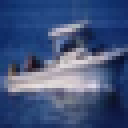
\includegraphics[width=1.05cm]{figs/o0.png}};
\node[lab, anchor=north] at (0.6,-2.16) {入力画像 $x$};
\draw[->] (1.2,-1.55) -- node[above, lab] {$+\sigma_1\varepsilon$} (1.87,-1.55);
% the blocks of the denoiser, left edge / height: encoder (32, 32, 16, 16, 8, 8), decoder (8, U at 8, 16, X at 16), then two blocks at 32
% that are not computed.  One red tick per block up to X: one number per block (the amplitude), collected on the red line.
\def\ybus{-2.68}
\foreach \xl/\h in {1.95/1.8, 2.22/1.8, 2.57/1.25, 2.84/1.25, 3.19/0.78, 3.46/0.78, 3.81/0.78, 4.08/0.78, 4.43/1.25, 4.70/1.25}{
  \draw[redc, line width=0.5pt] ({\xl+0.1},{-1.55-\h/2}) -- ({\xl+0.1},\ybus);
  \fill[redc] ({\xl+0.1},\ybus) circle (0.035);}
\foreach \xl/\h in {1.95/1.8, 2.22/1.8, 2.57/1.25, 2.84/1.25, 3.19/0.78, 3.46/0.78, 3.81/0.78, 4.43/1.25}
  \draw[black, fill=white, line width=0.7pt] (\xl,{-1.55-\h/2}) rectangle ++(0.2,\h);
\draw[navyc, fill=navyc!35, line width=0.9pt] (4.08,-1.94) rectangle ++(0.2,0.78);
\draw[redc, fill=redc!25, line width=0.9pt] (4.70,-2.175) rectangle ++(0.2,1.25);
\foreach \xl in {5.05, 5.32}
  \draw[black!45, densely dashed, line width=0.5pt] (\xl,-2.45) rectangle ++(0.2,1.8);
\draw[redc, line width=0.5pt] (2.05,\ybus) -- (4.80,\ybus);
\node[lab, anchor=south] at (2.8,-0.6) {エンコーダ};
\node[lab, anchor=south west] at (4.34,-0.6) {デコーダ};
\node[lab, anchor=south east, text=navyc] at (4.15,-1.15) {\textbf{U}};
\node[lab, anchor=south, text=redc] at (4.80,-0.92) {\textbf{X}};
\node[lab, anchor=north west, text=black!60] at (4.98,-2.5) {計算しない};
\node[lab, anchor=north west, align=left] at (0.0,-2.98) {凍結したノイズ除去器\\\textcolor{navyc}{\textbf{U}}：正立ブロック\\\textcolor{redc}{\textbf{X}}：打ち切りブロック};
% the two descriptors
\node[draw=navyc, rounded corners=2pt, line width=0.8pt, inner sep=3pt, align=left, font=\figlab, text width=21mm, anchor=north west] (fbox) at (6.1,-0.45)
  {$f$：U の出力の,\\チャネルごとの\\平均と標準偏差};
\node[draw=redc, rounded corners=2pt, line width=0.8pt, inner sep=3pt, align=left, font=\figlab, text width=21mm, anchor=north west] (zbox) at (6.1,-2.92)
  {$z$：X までの\\各ブロックの出力から\\数値を1つずつ};
\draw[->, navyc, line width=0.7pt] (4.18,-1.16) -- (4.18,-0.12) -- (7.2,-0.12) -- (7.2,-0.45);
\draw[->, redc, line width=0.7pt] (3.425,\ybus) -- (3.425,-3.43) -- (6.1,-3.43);
%% ================================================================ (b) the banks
\node[ttl] at (8.75,0.15) {\textbf{(b)}\ 事前：8通りの向き};
\draw[black!45, rounded corners=3pt] (8.75,-0.15) rectangle (12.25,-4.38);
\foreach \k/\xc/\yc in {1/10.11/-0.74, 2/10.89/-0.74, 3/11.67/-0.74, 4/9.33/-1.52, 5/10.11/-1.52, 6/10.89/-1.52, 7/11.67/-1.52}
  \node[inner sep=0, draw=black!55, line width=0.5pt] at (\xc,\yc) {\includegraphics[width=0.7cm]{figs/o\k.png}};
\node[inner sep=0, draw=navyc, line width=1.5pt] at (9.33,-0.74) {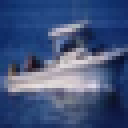
\includegraphics[width=0.7cm]{figs/o0.png}};
\draw[navyc, line width=1.0pt] (8.98,-2.31) rectangle ++(0.15,0.15);
\node[lab, anchor=west, align=left, text=navyc] at (9.2,-2.37) {そのまま(正立)の $N$ 枚\\→ バンク $u$};
\draw[black!55, line width=0.6pt] (8.98,-3.08) rectangle ++(0.15,0.15);
\node[lab, anchor=west, align=left, text=black!75] at (9.2,-3.14) {向きを変えた $7N$ 枚\\→ バンク $o$};
\node[lab, anchor=west, text=black!60] at (8.95,-3.95) {ノイズ $\varepsilon$ は変換しない};
%% ================================================================ (c) the score
\node[ttl] at (12.55,0.15) {\textbf{(c)}\ 2つのバンクへの近さを読む};
\draw[black!45, rounded corners=3pt] (12.55,-0.15) rectangle (17.6,-4.38);
% the two banks, the two circles and the input: written by gen/mk_schem.py in the coordinates of the panel
\begin{scope}[shift={(12.55,-0.15)}]
% written by gen/mk_schem.py: the two banks of Figure 1 (c), drawn for R = 1 (6 navy dots = u, 42 grey squares = o)
\foreach \p in {(1.612,-1.083),(1.380,-1.980),(1.120,-0.480),(0.780,-1.220),(0.380,-0.620),(0.360,-1.820)} \fill[navyc] \p circle (0.055);
\foreach \p in {(3.027,-1.223),(3.091,-1.535),(3.077,-0.925),(3.112,-1.790),(2.997,-0.662),(3.236,-1.128),(3.056,-2.008),(3.240,-2.415),(3.259,-2.064),(3.496,-2.116),(3.523,-0.975),(3.537,-0.342),(3.541,-1.408),(3.551,-1.697),(3.564,-2.415),(3.796,-2.094),(3.827,-0.968),(3.833,-1.304),(3.866,-0.601),(3.866,-0.255),(3.885,-1.756),(3.896,-2.420),(4.161,-0.666),(4.170,-1.307),(4.175,-0.324),(4.181,-2.452),(4.182,-1.657),(4.203,-2.001),(4.431,-2.376),(4.454,-1.760),(4.506,-1.039),(4.520,-1.347),(4.522,-2.001),(4.523,-0.244),(4.529,-0.644),(4.775,-0.620),(4.789,-0.342),(4.801,-2.352),(4.814,-1.411),(4.826,-1.728),(4.845,-1.059),(4.846,-2.002)} \fill[black!45] \p ++(-0.04,-0.04) rectangle ++(0.08,0.08);
\draw[navyc, line width=0.6pt] (2.150,-1.300) circle (0.580);
\draw[black!60, densely dashed, line width=0.6pt] (2.150,-1.300) circle (1.150);
\draw[navyc, line width=0.6pt] (2.150,-1.300) -- node[pos=0.62, above right, inner sep=1pt, text=navyc, font=\figlab] {$r^{u}_{R}$} (1.612,-1.083);
\draw[black!65, line width=0.6pt] (2.150,-1.300) -- node[pos=0.80, below left, inner sep=0.5pt, text=black!75, font=\figlab] {$r^{o}_{R}$} (3.056,-2.008);
\node[star, star points=5, star point ratio=2.2, fill=redc, inner sep=1.2pt] at (2.150,-1.300) {};

\end{scope}
\fill[navyc] (12.8,-2.80) circle (0.055); \node[lab, anchor=west, text=navyc] at (12.9,-2.80) {正立の train 画像($u$)};
\node[star, star points=5, star point ratio=2.2, fill=redc, inner sep=0.95pt] at (15.85,-2.80) {}; \node[lab, anchor=west] at (15.97,-2.80) {入力};
\fill[black!45] (12.75,-3.12) rectangle ++(0.1,0.1); \node[lab, anchor=west, text=black!75] at (12.9,-3.07) {向きを変えた train 画像($o$)};
\node[draw=black, rounded corners=2pt, line width=0.9pt, inner sep=3pt, align=left, font=\figlab, text width=45mm, anchor=north] at (15.075,-3.27)
  {密度：$r^{u}_{R}$ が小さいほど高い\\比：$r^{o}_{R}/r^{u}_{R}$ が大きいほど高い\\$s(x)=J_f(x)+J_z(x)$\ \ [式~(\ref{eq:J}),\,(\ref{eq:score})]};
\end{tikzpicture}
\end{adjustbox}
\caption{\method{} の概要. (a) テスト時は, 凍結したノイズ除去器の1回の順伝播を打ち切りブロック X で止め, 正立ブロック U の出力の平均と標準偏差 $f$ と, X までの各ブロックの出力から数値を1つずつ読んだ並び $z$ を求める. (b) 事前に, train 画像を8通りの向きで同じように通し, そのまま(正立)の $N$ 枚をバンク $u$, 向きを変えた $7N$ 枚をバンク $o$ とする. (c) 記述子ごとに, $u$ の $R$ 番目の最近傍までの距離 $r^{u}_{R}$ と, $o$ の $7R$ 番目の最近傍までの距離 $r^{o}_{R}$ から, 密度と比を読んで足す(図は $R=1$ の場合). ブロックの数と点の配置は模式的なものである.}
\label{fig:method}
\end{figure*}

ところが, チャネルごとの統計量は特徴マップの位置を並べ替えても変わらないので, 画像の向きの情報が弱い. 内容は分布内と同じで向きだけが異なる「上下反転した分布内の画像」は, CFS の kNN ヘッドでも, 平均\nPriorUdT\%でしか見分けられない(\ref{sec:main}節). 向きを補う素直な方法は, 回転や鏡像を当てる分類器を学習することである~\cite{golan2018geometric,hendrycks2019ss,tack2020csi}. しかし, それは勾配による学習と追加のネットワークを持ち込み, 学習済みのモデルを凍結したまま使えるという利点を損なう.

本研究は, 学習を一切行わずに向きまで測る. 鍵は, 向きを変えた train 画像を, 近傍を探す相手に加えることである(図~\ref{fig:method}). train 画像を8通りの向き(4つの回転と, その鏡像)でノイズ除去器に通しておけば, 入力が正立の train 画像と向きを変えた train 画像のどちらに近いかは, それぞれの最近傍までの距離を比べるだけで読める. 2つの距離の比の対数は, kNN による密度比の推定~\cite{wang2009divergence}であり, 入力が正立である事後確率のオッズにあたる. これを, 向きを最もよく見分けるブロック(正立ブロック)の平均と標準偏差 $f$ と, 各ブロックの出力から数値を1つだけ読んだ並び $z$ の, 2つの記述子で読む. スコアは, 記述子ごとに「正立の train 画像の密度の対数」と「正立と向き替えの密度の比の対数」を足したもので, 重みも, 学習するパラメータもない. 記述子を読み終えたブロックで, 順伝播を打ち切る. これを \method{} と呼ぶ.

5つの分布内データセットの51組で, 自然画像の分布外集合での平均 AUROC は\nOursT\%であり, 同じ拡散モデルを用いる先行研究の最良(CFS の kNN ヘッド, \nPriorT\%)を\nGapPriorT{}ポイント上回る. 比の代わりに, 回転と鏡像を当てる2つの分類器を学習して用いる構成(\nTrainedT\%)も下回らない. 順伝播の計算時間は, 1回の順伝播の\nPassX{}倍である(記述子の計算とバンクの探索を含めても\nAllX{}倍). 本研究の貢献は次の3つである.
\begin{itemize}
\setlength{\itemsep}{0pt}\setlength{\parskip}{0pt}
\item 向きを変えた train 画像をバンクに加え, 最近傍までの距離の比で向きを読むスコア. 勾配による学習も, 追加のネットワークも, ラベルも, 分布外の画像も用いない.
\item 51組で同じ拡散モデルを用いる先行研究の最良を, CFS の評価手順の12組で文献の公表値の最良を上回ること. 順伝播は, 途中で打ち切る1回である.
\item 学習した分類器を用いる構成との比較と, 各部分の寄与の分析. 上下反転と鏡像の検知が学習した分類器に及ばないという限界も示す.
\end{itemize}

\section{関連研究}
\label{sec:related}
\textbf{拡散モデルによる分布外検知.} 深層生成モデルは, 分布外の画像に分布内より高い尤度を与えることがある~\cite{nalisnick2019deep}. これに対し, 典型集合による検定~\cite{nalisnick2019typ}, 入力の複雑さによる補正~\cite{serra2020input}, 複数のスケールでのスコアの大きさ~\cite{mahmood2021msma}, 再構成の誤差~\cite{graham2023ddpmood}, 生成の軌跡の統計量~\cite{heng2024diffpath}, 変換に対する事後平均の一貫性~\cite{alexis2026gepc}, 事後共分散の固有値~\cite{shoushtari2026eigenscore}, スコアの大きさと曲率~\cite{barkley2026scoped}, 局所的な内在次元~\cite{kamkari2024geometric}が提案されているが, 多くは1枚あたり数回から数百回のネットワークの評価を要する. CFS~\cite{rouzoumka2026cfs}は, 低いノイズで1回通した中間特徴を, 対角ガウスや, 識別的な分類器の特徴について提案された kNN~\cite{sun2022knn}で判定する. 本研究は同種の特徴を用いるが, 近傍を探す相手に向きを変えた train 画像を加える点と, ブロックごとに数値を1つだけ読んだ並びを第2の記述子とする点が異なる.

\textbf{向きと密度比.} 画像の回転などの幾何変換を当てる分類器を分布内のデータで学習する方法~\cite{golan2018geometric,hendrycks2019ss}や, 回転した画像を別の画像として扱う対照学習~\cite{tack2020csi}は, 向きを変えた画像を学習に用いる(鏡像にも向きの手がかりが残る~\cite{lin2020chirality}). 本研究は, 学習には用いず, 近傍を探すバンクに加えるだけである. また, 背景を表すモデルとの尤度比~\cite{ren2019likelihood}や補助の外れ値データ~\cite{hendrycks2019oe}は, 分布内らしさを別の分布と比べて測る. 本研究の比は, 「向きを変えた分布内の画像」を比べる相手とする密度比を, 2つの標本への最近傍の距離の比~\cite{wang2009divergence,sugiyama2012density}で推定するものであり, 別のモデルも外れ値データも要らない.

\section{準備}
\label{sec:prep}
\textbf{問題設定.} 分布内の画像の密度を $p(x)$ とし, そこから得られた $N$ 枚の train 画像 $x_1,\ldots,x_N$ が与えられる. 入力画像 $x$ に分布内らしさを表すスコア $s(x)$ を与え, しきい値より小さい入力を分布外と判定する. 評価の指標は AUROC であり, 分布内の画像の95\%を残すときに分布外の画像が通過する割合(FPR95)も示す.

\textbf{ノイズ除去器の中間特徴.} 拡散モデルのノイズ除去器は, ノイズを加えた画像から元の画像を推定するネットワークであり, 多くは, エンコーダで解像度を下げてデコーダで上げる U-Net~\cite{ronneberger2015unet}である. 入力側から数えて $h$ 番目のブロックの出力(特徴マップ)の, チャネル $c$, 位置 $(i,j)$ の値を $h_{c,i,j}$ と書く. 画像 $x$ に小さなノイズ $\sigma_1\varepsilon$ ($\sigma_1=0.01$. $\varepsilon$ はすべての画像に共通の1枚)を加えて, ノイズ除去器に1回通す.

\textbf{kNN による密度の推定.} 入力の特徴から, $N$ 個の train 画像の特徴のうち $R$ 番目に近いものまでの距離を $r_R(x)$ とする. 特徴が $d$ 次元の広がりをもつとき, 半径 $r_R(x)$ の球の体積は $V r_R(x)^{d}$ ($V$ は半径1の球の体積)であり, そこに $N$ 個のうち $R$ 個が入っているので, 密度は
\begin{equation}
\hat{p}(x)=\frac{R}{N V\, r_R(x)^{d}}
\label{eq:knn}
\end{equation}
と推定できる~\cite{loftsgaarden1965knn}. その対数は, 定数を除いて $-d\log r_R(x)$ に等しい.

\section{提案手法：\method}
\label{sec:method}
train 画像と, それで学習した拡散モデルのノイズ除去器だけを用いる. 勾配で学習するものも, 当てはめる分類器もなく, train 画像から求めるのは, バンクのほかには平均, 標準偏差, 次元といった統計量だけである.

\subsection{2つの記述子}
1回の順伝播から, 2つの記述子を読む(図~\ref{fig:method}a). 第1の記述子 $f(x)$ は, 正立ブロック U (\ref{sec:blocks}節)の出力の, チャネルごとの位置についての平均と標準偏差を並べ, 長さ1に正規化したベクトルである. 距離には, 単位球面上の2点を結ぶ弦の長さを用いる.

第2の記述子は, ブロックごとに数値を1つだけ読む. ブロック $h$ の出力の, チャネル $c$ の位置についての平均を $\mu_c$, チャネルの数を $C_h$ として,
\begin{equation}
a_h(x)=\frac{1}{C_h}\sum_{c=1}^{C_h}\log\max_{i,j}\,\bigl|h_{c,i,j}-\mu_c\bigr|
\label{eq:amp}
\end{equation}
を振幅と呼ぶ. チャネルごとに, 平均から最も外れた値の大きさの対数をとり, チャネルについて平均したものである. 入力側から打ち切りブロック X (\ref{sec:blocks}節)までの振幅を, ブロックごとに正立の train 画像での平均 $\bar{a}_h$ と標準偏差 $\mathrm{sd}_h$ でそろえて並べ,
\begin{equation}
z(x)=\Bigl(\frac{a_1(x)-\bar{a}_1}{\mathrm{sd}_1},\,\ldots,\,\frac{a_{\mathrm{X}}(x)-\bar{a}_{\mathrm{X}}}{\mathrm{sd}_{\mathrm{X}}}\Bigr)
\label{eq:z}
\end{equation}
とする. 距離はユークリッド距離である. $z$ の長さは分布内データセットごとに\nNzMin{}から\nNzMax{}であり, $f$ (数百から千次元)よりずっと短い.

\begin{figure}[t]\centering
\begin{adjustbox}{max width=\columnwidth}% written by gen/mk_schem.py -- Figure 2: what the two readings see (schematic, drawn for R = 1; natural width about 8.3 cm).
%   The same two banks in three panels: 6 navy dots = the upright train images (u), 42 grey squares = the train images in the seven
%   other orientations (o).  The input (red star): (i) an ID image, (ii) an image whose orientation alone differs, (iii) an image whose
%   content differs.  The solid circle passes through the nearest entry of u, the dashed circle through the 7th nearest entry of o.
\begin{tikzpicture}[font=\figlab, line join=round, line cap=round, lab/.style={font=\figlab, inner sep=1pt, align=center}]
\begin{scope}[shift={(0.00,0)}]
  \draw[black!40, rounded corners=2pt] (0,0) rectangle (2.62,-2.3);
  \foreach \p in {(0.420,-0.500),(0.800,-0.580),(0.280,-0.980),(0.660,-1.120),(0.980,-0.950),(0.550,-1.520)} \fill[navyc] \p circle (0.045);
  \foreach \p in {(1.487,-0.346),(1.531,-0.508),(1.538,-0.743),(1.495,-0.909),(1.507,-1.142),(1.459,-1.335),(1.507,-1.616),(1.683,-0.279),(1.657,-0.555),(1.685,-0.754),(1.656,-0.924),(1.709,-1.149),(1.733,-1.377),(1.686,-1.582),(1.864,-0.365),(1.870,-0.572),(1.871,-0.719),(1.873,-0.953),(1.919,-1.204),(1.865,-1.403),(1.875,-1.591),(2.063,-0.298),(2.108,-0.501),(2.107,-0.762),(2.065,-0.925),(2.044,-1.182),(2.036,-1.354),(2.074,-1.541),(2.304,-0.278),(2.242,-0.540),(2.215,-0.726),(2.273,-0.941),(2.276,-1.162),(2.287,-1.357),(2.256,-1.604),(2.479,-0.318),(2.477,-0.554),(2.421,-0.776),(2.472,-0.923),(2.420,-1.144),(2.414,-1.380),(2.463,-1.575)} \fill[black!45] \p ++(-0.03,-0.03) rectangle ++(0.06,0.06);
  \begin{scope} \clip (0.01,-0.01) rectangle (2.6100000000000003,-2.29);
    \draw[navyc, line width=0.6pt] (0.620,-0.860) circle (0.263);
    \draw[black!60, densely dashed, line width=0.6pt] (0.620,-0.860) circle (1.038);
  \end{scope}
  \node[star, star points=5, star point ratio=2.2, fill=redc, inner sep=1.0pt] at (0.620,-0.860) {};
\end{scope}
\begin{scope}[shift={(2.82,0)}]
  \draw[black!40, rounded corners=2pt] (0,0) rectangle (2.62,-2.3);
  \foreach \p in {(0.420,-0.500),(0.800,-0.580),(0.280,-0.980),(0.660,-1.120),(0.980,-0.950),(0.550,-1.520)} \fill[navyc] \p circle (0.045);
  \foreach \p in {(1.487,-0.346),(1.531,-0.508),(1.538,-0.743),(1.495,-0.909),(1.507,-1.142),(1.459,-1.335),(1.507,-1.616),(1.683,-0.279),(1.657,-0.555),(1.685,-0.754),(1.656,-0.924),(1.709,-1.149),(1.733,-1.377),(1.686,-1.582),(1.864,-0.365),(1.870,-0.572),(1.871,-0.719),(1.873,-0.953),(1.919,-1.204),(1.865,-1.403),(1.875,-1.591),(2.063,-0.298),(2.108,-0.501),(2.107,-0.762),(2.065,-0.925),(2.044,-1.182),(2.036,-1.354),(2.074,-1.541),(2.304,-0.278),(2.242,-0.540),(2.215,-0.726),(2.273,-0.941),(2.276,-1.162),(2.287,-1.357),(2.256,-1.604),(2.479,-0.318),(2.477,-0.554),(2.421,-0.776),(2.472,-0.923),(2.420,-1.144),(2.414,-1.380),(2.463,-1.575)} \fill[black!45] \p ++(-0.03,-0.03) rectangle ++(0.06,0.06);
  \begin{scope} \clip (0.01,-0.01) rectangle (2.6100000000000003,-2.29);
    \draw[navyc, line width=0.6pt] (1.980,-0.950) circle (1.000);
    \draw[black!60, densely dashed, line width=0.6pt] (1.980,-0.950) circle (0.294);
  \end{scope}
  \node[star, star points=5, star point ratio=2.2, fill=redc, inner sep=1.0pt] at (1.980,-0.950) {};
\end{scope}
\begin{scope}[shift={(5.64,0)}]
  \draw[black!40, rounded corners=2pt] (0,0) rectangle (2.62,-2.3);
  \foreach \p in {(0.420,-0.500),(0.800,-0.580),(0.280,-0.980),(0.660,-1.120),(0.980,-0.950),(0.550,-1.520)} \fill[navyc] \p circle (0.045);
  \foreach \p in {(1.487,-0.346),(1.531,-0.508),(1.538,-0.743),(1.495,-0.909),(1.507,-1.142),(1.459,-1.335),(1.507,-1.616),(1.683,-0.279),(1.657,-0.555),(1.685,-0.754),(1.656,-0.924),(1.709,-1.149),(1.733,-1.377),(1.686,-1.582),(1.864,-0.365),(1.870,-0.572),(1.871,-0.719),(1.873,-0.953),(1.919,-1.204),(1.865,-1.403),(1.875,-1.591),(2.063,-0.298),(2.108,-0.501),(2.107,-0.762),(2.065,-0.925),(2.044,-1.182),(2.036,-1.354),(2.074,-1.541),(2.304,-0.278),(2.242,-0.540),(2.215,-0.726),(2.273,-0.941),(2.276,-1.162),(2.287,-1.357),(2.256,-1.604),(2.479,-0.318),(2.477,-0.554),(2.421,-0.776),(2.472,-0.923),(2.420,-1.144),(2.414,-1.380),(2.463,-1.575)} \fill[black!45] \p ++(-0.03,-0.03) rectangle ++(0.06,0.06);
  \begin{scope} \clip (0.01,-0.01) rectangle (2.6100000000000003,-2.29);
    \draw[navyc, line width=0.6pt] (1.220,-2.030) circle (0.842);
    \draw[black!60, densely dashed, line width=0.6pt] (1.220,-2.030) circle (0.933);
  \end{scope}
  \node[star, star points=5, star point ratio=2.2, fill=redc, inner sep=1.0pt] at (1.220,-2.030) {};
\end{scope}
\node[lab, anchor=south] at (1.31,0.05) {\textbf{(i)}\ 分布内の画像};
\node[lab, anchor=south] at (4.13,0.05) {\textbf{(ii)}\ 向きだけが異なる画像};
\node[lab, anchor=south] at (6.95,0.05) {\textbf{(iii)}\ 内容が異なる画像};
\node[lab, anchor=north, align=center] at (1.31,-2.36) {$u$ に近く, $o$ から遠い\\密度：高い,\ 比：高い};
\node[lab, anchor=north, align=center] at (4.13,-2.36) {$u$ より $o$ に近い\\\textcolor{redc}{比：低い}};
\node[lab, anchor=north, align=center] at (6.95,-2.36) {$u$ からも $o$ からも遠い\\\textcolor{redc}{密度：低い}};
\fill[navyc] (0.12,-3.28) circle (0.045); \node[lab, anchor=west, text=navyc] at (0.2,-3.28) {正立の train 画像($u$)};
\fill[black!45] (2.72,-3.31) rectangle ++(0.06,0.06); \node[lab, anchor=west, text=black!75] at (2.84,-3.28) {向きを変えた train 画像($o$)};
\node[star, star points=5, star point ratio=2.2, fill=redc, inner sep=0.9pt] at (6.2,-3.28) {}; \node[lab, anchor=west] at (6.3,-3.28) {入力};
\end{tikzpicture}
\end{adjustbox}
\caption{密度と比が見るもの(模式図, $R=1$ の場合). 実線の円は正立の train 画像の最も近い要素を, 破線の円は向きを変えた train 画像の7番目に近い要素を通る. (i) 分布内の画像は $u$ に近く, $o$ から遠い. (ii) 向きだけが異なる画像は $o$ のほうに近く, 比が下がる. (iii) 内容が異なる画像は $u$ から遠く, 密度が下がる.}
\label{fig:idea}
\end{figure}

\subsection{8通りの向きのバンク}
正方形の画像を自分自身に重ねる変換は, 4つの回転と, 左右反転をしてから回転する4通りの, 計8通りである. その集合を $\mathcal{D}$, 恒等変換を除く7通りを $\mathcal{D}^{*}$ と書く. 事前に, train 画像 $x_1,\ldots,x_N$ と, それを変換した $\Dm x_i$ ($\Dm\in\mathcal{D}^{*}$)を, テスト時と同じノイズと打ち切りでノイズ除去器に通し, 記述子を求めておく(図~\ref{fig:method}b). ノイズは回転も反転もしない. そのままの $N$ 枚の記述子の集まりを正立のバンク $u$, 向きを変えた $7N$ 枚の記述子の集まりを向き替えのバンク $o$ と呼ぶ. 分布内に標準の向きがあれば, $\Dm x_i$ は分布内にほとんど現れない画像であり, バンク $o$ は「内容は分布内と同じで, 分布内ではない画像」の見本になる.

\subsection{密度と, 向きの比}
記述子 $g\in\{f,z\}$ のそれぞれについて, $g(x)$ から, バンク $u$ の $R$ 番目に近い要素までの距離を $r^{u}_{R}(x)$, バンク $o$ の $7R$ 番目に近い要素までの距離を $r^{o}_{R}(x)$ とする. $o$ は $u$ の7倍の要素をもつので, どちらの球にも, バンクの要素の $R/N$ が入る. 式~\eqref{eq:knn}により, 2つのバンクのもとの分布の密度 $p_u$, $p_o$ は, 共通の定数 $\kappa$ を用いて
\begin{equation}
\log\hat{p}_u(x)=-d\log r^{u}_{R}(x)+\kappa
\label{eq:pu}
\end{equation}
\begin{equation}
\log\hat{p}_o(x)=-d\log r^{o}_{R}(x)+\kappa
\label{eq:po}
\end{equation}
と推定でき, 差をとると, 密度の比の対数が距離の比の対数になる.
\begin{equation}
\log\frac{\hat{p}_u(x)}{\hat{p}_o(x)}=d\,\bigl\{\log r^{o}_{R}(x)-\log r^{u}_{R}(x)\bigr\}
\label{eq:ratio}
\end{equation}
これは, 2つの標本への最近傍の距離から分布の隔たりを推定する方法~\cite{wang2009divergence}で, 1点ごとに足し合わされる量である.

\textbf{比の意味.} 正立の分布内画像を, 8通りの向きに等確率で変換した画像の混合を考える. この混合のもとで, 記述子の値が $g(x)$ である画像が変換されていない(正立である)事後確率は, ベイズの定理により $p_u(x)/\{p_u(x)+7p_o(x)\}$ であり, そのオッズの対数は
\begin{equation}
\log\frac{P(\text{正立}\mid x)}{1-P(\text{正立}\mid x)}=\log\frac{p_u(x)}{p_o(x)}-\log 7
\label{eq:odds}
\end{equation}
である. 式~\eqref{eq:ratio}は, 定数を除いて, 入力が正立であるオッズを最近傍の距離だけで読んだものであり, 回転や鏡像を当てる分類器が学習によって求める事後確率を, 学習なしに置き換える.

\textbf{2つを足す.} 密度 [式~\eqref{eq:pu}]は, 入力が正立の train 画像に近いかを表し, 内容が異なる画像で下がる. 比 [式~\eqref{eq:ratio}]は, 入力が向きを変えた train 画像より正立の train 画像に近いかを表し, 向きだけが異なる画像で下がる(図~\ref{fig:idea}. 実際の値は補足資料の図~\ref{fig:scatter}). 分布外の入力はあらかじめ分からないので, 2つを足す.

\subsection{スコア}
\label{sec:score}
$\ell^{u}_{R}(x)=-\log r^{u}_{R}(x)$, $\ell^{o}_{R}(x)=-\log r^{o}_{R}(x)$ と書く. 式~\eqref{eq:pu}と式~\eqref{eq:ratio}の和は, 定数を除いて $d\,\{2\ell^{u}_{R}(x)-\ell^{o}_{R}(x)\}$ である. 近傍の順位 $R$ は, 分布外の画像を使わずに決める. train 画像での $2\ell^{u}_{R}-\ell^{o}_{R}$ の平均を $m_R$ として,
\begin{equation}
J_g(x)=d_g\min_{R}\bigl\{2\ell^{u}_{R}(x)-\ell^{o}_{R}(x)-m_R\bigr\}
\label{eq:J}
\end{equation}
とする. $R$ は1から1000までの10通り(1, 2, 5, 10, 20, 50, 100, 200, 500, 1000)である. 小さい $R$ はごく近くの train 画像との近さを, 大きい $R$ は広い範囲での密度を見る. $m_R$ を引いて水準をそろえたうえで, その画像が最も分布内らしくない値をとる. $m_R$ は, train 画像から選んだ5000枚について, その画像自身とその7通りの変換をバンクから除いて求める. スコアは, 2つの記述子の和
\begin{equation}
s(x)=J_f(x)+J_z(x)
\label{eq:score}
\end{equation}
である. 重みは調整しない. 2つの項の交換比は, 次元 $d_f$ と $d_z$ が決める.

\textbf{次元.} $d$ 次元の広がりでは, $R$ 番目の最近傍までの距離が $R^{1/d}$ に比例して伸びるので, train 画像での $\ell^{u}_{R}$ の平均は, $\log R$ に対して傾き $-1/d$ の直線になる. そこで $d_g$ を, $R=1$ から20までの5点に当てはめた直線の傾きの逆数の符号を変えたものとする. 分布内データセットごとに, $d_f$ は\nDimFMin{}から\nDimFMax, $d_z$ は\nDimZMin{}から\nDimZMax{}である.

\textbf{密度と比を別々に読む場合.} 分析のために, 密度だけを同じ読み方で求めた $T_g=d_g\min_R\{\ell^{u}_{R}-m^{T}_{R}\}$ と, 比だけを求めた $Q_g=d_g\min_R\{\ell^{u}_{R}-\ell^{o}_{R}-m^{Q}_{R}\}$ も用いる($m^{T}_{R}$, $m^{Q}_{R}$ は, それぞれの中身の train 画像での平均). $T_f$ は, 正立ブロックの特徴だけで判定する kNN にあたる.

\subsection{正立ブロックと打ち切りブロック}
\label{sec:blocks}
\textbf{正立ブロック.} $f$ を読むブロックは, 向きを最もよく見分けるブロックとする. ブロック $b$ の出力の平均と標準偏差を記述子としたときの, 正立のバンクへの $R$ 番目の最近傍の距離の対数の符号を変えたものを $\ell_{b,R}$ とする. train 画像から選んだ5000枚 $x'_1,\ldots,x'_M$ について, そのままの画像と, 変換した画像を $\ell_{b,R}$ で見分ける AUROC の平均
\begin{equation}
\begin{split}
A_{b,R}=\frac{1}{7}\sum_{\Dm\in\mathcal{D}^{*}}\mathrm{AUROC}\bigl[&\{\ell_{b,R}(x'_j)\}_{j},\\
&\{\ell_{b,R}(\Dm x'_j)\}_{j}\bigr]
\end{split}
\label{eq:A}
\end{equation}
を求め(その画像自身は近傍から除く), $\max_R A_{b,R}$ が最大のブロックを正立ブロック U とする. 入力に近いブロックと出力に近いブロックは, 画像を回転・反転しても特徴マップが同じように回転・反転するだけで, 平均と標準偏差は向きを区別しない. そのあいだのブロックは, 画像の広い範囲をまとめて見るので, 分布内の画像に多い配置に合わせた応答をもち, 向きを区別する. 選ばれるのは, 4つの分布内でデコーダの $8{\times}8$ のブロック, FashionMNIST でエンコーダの $8{\times}8$ のブロックである(補足資料の表~\ref{tab:models}).

\textbf{打ち切りブロック.} 向きを変えたときの振幅のずれは, 解像度の低いブロックから現れ, 正立ブロックより先のデコーダのブロックで大きい(\ref{sec:what}節). そこで $z$ は, 正立ブロックの2倍の解像度をもつデコーダのブロックのうち, 最後のものまで読む. これを打ち切りブロック X と呼び, 順伝播はここで止める.

\section{実験}
\subsection{設定}
\textbf{データ.} 分布内データセットは, CIFAR-10, SVHN, CelebA, ImageNet-64, FashionMNIST の5つである. 公開されている学習済みの拡散モデル~\cite{karras2022edm,kamkari2024geometric,nichol2021improved,karras2024edm2}を変更せずに用い, FashionMNIST だけは本研究で学習した. 分布外の集合は, 他のデータセットの画像の集合(以下, 自然画像の分布外集合. 分布内ごとに9, 9, 9, 7, 4集合), 上下反転した分布内の画像, 合成画像(一様ノイズと定数画像. ImageNet-64 を除く)であり, 分布内との組は計51組である(一覧は補足資料の表~\ref{tab:pairst}). 左右反転した分布内の画像も調べる.

\textbf{画像の分け方.} 画像は, 互いに重ならない train, val1, val2, test 画像に分ける. train 画像(5万枚. ImageNet-64 は1万枚)は, バンクと, 正立ブロック, $d_g$, $m_R$ の計算に用いる. val1 画像は, 分布内の画像と, 評価に用いない分布外データセット(STL-10, GTSRB, Flowers-102 など)の画像であり, val2 画像は, 分布内と各分布外集合から取り分けた画像である. \method{} の記述子と順位の読み方は, この2つで定めた. 評価は test 画像(各集合500枚)で, 確定した手法について1回行った. ただし, test 画像は, 学習した分類器を用いる構成や, 本手法の以前の構成の評価にも用いてきた画像であり, 一度も見ていない画像ではない. 別に取り分けた画像での同じ評価は, 補足資料に示す.

\textbf{比較手法.} 同じ拡散モデルを用いる先行研究として, 尤度(NLL~\cite{song2021score}), 入力の複雑さによる補正(IC~\cite{serra2020input}. 符号長に PNG と JPEG2000 を用いる2通り), 典型集合による検定(TT~\cite{nalisnick2019typ}), MSMA 型~\cite{mahmood2021msma}, DiffPath~\cite{heng2024diffpath}, GEPC~\cite{alexis2026gepc}, EigenScore~\cite{shoushtari2026eigenscore}の8手法と, CFS~\cite{rouzoumka2026cfs}(対角ガウスと kNN ヘッドの2通り. 公式コードの手順で同じ拡散モデルと train 画像に当てはめた)の計10手法と比べる. 回転の予測~\cite{hendrycks2019ss}(train 画像で一から学習した ResNet-18)は, 拡散モデルを用いない参考として示す.

\textbf{評価.} AUROC は, 分布内の画像と分布外の集合1つとの組ごとに求め, 分布内データセットごとに, 自然画像の分布外集合について平均する. \method{}, CFS, GEPC, EigenScore は, 画像に加えるノイズ $\varepsilon$ を決める乱数の種3つの平均, ほかの手法は1回の値である. 手法どうしの比較では, 画像を復元抽出するブートストラップ~\cite{efron1979bootstrap}(2000回)で AUROC の差の95\%信頼区間を求め, それが0を含まず差が0.05ポイント以上のときを勝ち/負け, ほかを引き分けとする.

\begin{table*}[t]\centering\scriptsize\setlength{\tabcolsep}{3.2pt}\renewcommand{\arraystretch}{0.9}
\caption{比較手法との比較(AUROC, \%. test 画像, 各集合500枚). 左の5列：分布内ごとの, 自然画像の分布外集合の平均. 上下反転：上下反転した分布内の画像の, 5つの平均. FPR95：自然画像の分布外集合での5つの平均(低いほどよい). 勝/分/負：全51組での, \method{} のその行に対する結果. 上の10行が同じ拡散モデルを用いる先行研究で, 参考の行は順位づけしない. $\dagger$：先行研究の中の最良. \protect\colorbox{firstblue}{\textbf{水色の太字}}：\method{} がそれに並ぶか上回る列. 順伝播：1枚あたりの回数(+は逆伝播). $\ddagger$：途中で打ち切るので, 打ち切りまでの計算時間を1回の順伝播の時間で割った値(5つのモデルの平均).}
\label{tab:main}
\begin{adjustbox}{max width=\textwidth}\begin{tabular}{@{}lcccccccccc@{}}\toprule
& \multicolumn{5}{c}{分布内(自然画像の分布外集合の平均)} & & & & \method{} の & \\\cmidrule(lr){2-6}
手法 & CIFAR-10 & SVHN & CelebA & ImageNet-64 & FashionMNIST & 5つの平均 & 上下反転 & FPR95 & 勝/分/負 & 順伝播\\\midrule
\inputrows{tab_main.tex}
\end{tabular}\end{adjustbox}
\end{table*}

\subsection{比較手法との比較}
\label{sec:main}
表~\ref{tab:main}に結果を示す. 自然画像の分布外集合での平均 AUROC は, \method{} が\nOursT\%(95\%信頼区間\nOursLoT--\nOursHiT)で, 同じ拡散モデルを用いる先行研究の最良である CFS の kNN ヘッド(\nPriorT\%)を\nGapPriorT{}ポイント(\nGapPriorLoT--\nGapPriorHiT)上回る. 差は, 先行研究が飽和していない分布内で大きく, CIFAR-10 で\nOursCtenT{}対\nPriorBestCtenT\%, ImageNet-64 で\nOursInT{}対\nPriorBestInT\%である. FPR95 の平均は\nFprT\%で, 先行研究の最良(\nPriorFprT\%)の半分以下である. 上下反転した分布内の画像では\nUdT\%であり, 先行研究の最良(EigenScore, \nEigenUdT\%)を上回るが, 回転を当てる分類器を学習する回転の予測(\nRotUdT\%)には及ばない.

弱点は SVHN である. \method{} が先行研究のいずれかに負けた\nNLossPairs{}組のうち\nNLossSvhn{}組は, SVHN を分布内とする組であり(残りは ImageNet-64 に対する iNaturalist), SVHN を分布内とする平均(\nOursSvhnT\%)は DiffPath(\nPriorBestSvhnT\%)に及ばない(\ref{sec:limits}節).

\begin{table}[t]\centering\scriptsize\setlength{\tabcolsep}{1.8pt}\renewcommand{\arraystretch}{0.92}
\caption{各部分の寄与と, 順伝播を止める位置(test 画像, 5つの分布内の平均. AUROC と FPR95, \%). 自然：自然画像の分布外集合. 上下, 左右：その反転をした分布内の画像. 勝/分/負：全51組での, \method{} のその行に対する結果. $T_g$, $Q_g$：密度と比を別々に読んだもの(\ref{sec:score}節). 参考：比の代わりに, 学習した2つの MLP を用いる構成. 順伝播：表~\ref{tab:main}の $\ddagger$ と同じ.}
\label{tab:parts}
\begin{tabular}{@{}lcccccc@{}}\toprule
構成 & 自然 & 上下 & 左右 & FPR95 & 勝/分/負 & 順伝播\\\midrule
\inputrows{tab_parts.tex}
\end{tabular}
\end{table}

\begin{figure*}[t]\centering
% written by gen/mk.py from data/fig_small.json (test images, noise seed 0)
\begin{tikzpicture}
\begin{groupplot}[group style={group size=5 by 1, horizontal sep=8mm}, width=41mm, height=32mm, unbounded coords=jump,
  tick label style={font=\figlab}, title style={font=\scriptsize, yshift=-1.5mm, text height=1.6ex, text depth=0.3ex}, xlabel style={font=\figlab}, ylabel style={font=\figlab}, xlabel={ブロック(入力側 $\rightarrow$ 出力側)}, every axis plot/.append style={line width=0.7pt},
  legend style={font=\figlab, draw=none, fill=none, legend columns=4, /tikz/every even column/.append style={column sep=3mm}}]
\nextgroupplot[title={CIFAR-10}, ylabel={振幅(標準偏差を単位)}, legend to name=profleg]
\draw[navyc!70, densely dotted, line width=0.6pt] (axis cs:21,\pgfkeysvalueof{/pgfplots/ymin}) -- (axis cs:21,\pgfkeysvalueof{/pgfplots/ymax}) node[pos=0.93, right, inner sep=1pt, font=\figlab, text=navyc] {U};
\draw[redc!80, densely dotted, line width=0.6pt] (axis cs:28,\pgfkeysvalueof{/pgfplots/ymin}) -- (axis cs:28,\pgfkeysvalueof{/pgfplots/ymax}) node[pos=0.78, left, inner sep=1pt, font=\figlab, text=redc] {X};
\addplot[navyc] coordinates {(1,-0.01) (2,0.01) (3,0.04) (4,0.03) (5,0.05) (6,-0.02) (7,-0.02) (8,-0.01) (9,-0.06) (10,-0.04) (11,-0.08) (12,-0.09) (13,-0.15) (14,-0.15) (15,-0.03) (16,0.0) (17,0.0) (18,-0.01) (19,-0.12) (20,-0.21) (21,-0.22) (22,-0.18) (23,-0.17) (24,-0.15) (25,-0.19) (26,-0.2) (27,-0.21) (28,-0.18)};
\addplot[redc] coordinates {(1,-0.01) (2,0.01) (3,0.04) (4,0.05) (5,0.06) (6,-0.03) (7,-0.08) (8,-0.19) (9,-0.36) (10,-0.42) (11,-0.62) (12,-0.79) (13,-1.04) (14,-1.06) (15,-0.2) (16,-0.09) (17,-0.12) (18,-0.12) (19,-0.69) (20,-1.45) (21,-1.91) (22,-1.9) (23,-1.91) (24,-1.79) (25,-1.83) (26,-1.81) (27,-1.67) (28,-1.34)};
\addplot[redc, densely dashed] coordinates {(1,-0.0) (2,-0.0) (3,-0.01) (4,-0.0) (5,-0.02) (6,-0.0) (7,-0.1) (8,-0.28) (9,-0.5) (10,-0.52) (11,-0.65) (12,-0.78) (13,-0.96) (14,-1.03) (15,-0.38) (16,-0.24) (17,-0.31) (18,-0.18) (19,-0.72) (20,-1.37) (21,-1.82) (22,-1.87) (23,-1.88) (24,-1.61) (25,-1.67) (26,-1.66) (27,-1.54) (28,-1.25)};
\addplot[black] coordinates {(1,-0.35) (2,-0.32) (3,-0.28) (4,-0.27) (5,-0.08) (6,-0.41) (7,-0.68) (8,-0.9) (9,-0.69) (10,-1.0) (11,-1.3) (12,-1.4) (13,-1.43) (14,-1.3) (15,-1.26) (16,-1.31) (17,-1.39) (18,-1.25) (19,-1.46) (20,-1.78) (21,-2.25) (22,-2.61) (23,-2.59) (24,-1.96) (25,-1.85) (26,-1.81) (27,-2.09) (28,-1.68)};
\legend{分布内の画像, 上下反転した分布内の画像, 向きを変えた train 画像(7 通り), 自然画像の分布外集合(平均)}
\nextgroupplot[title={SVHN}]
\draw[navyc!70, densely dotted, line width=0.6pt] (axis cs:10,\pgfkeysvalueof{/pgfplots/ymin}) -- (axis cs:10,\pgfkeysvalueof{/pgfplots/ymax}) node[pos=0.93, right, inner sep=1pt, font=\figlab, text=navyc] {U};
\draw[redc!80, densely dotted, line width=0.6pt] (axis cs:11,\pgfkeysvalueof{/pgfplots/ymin}) -- (axis cs:11,\pgfkeysvalueof{/pgfplots/ymax}) node[pos=0.78, left, inner sep=1pt, font=\figlab, text=redc] {X};
\addplot[navyc] coordinates {(1,-0.32) (2,-0.14) (3,0.06) (4,0.1) (5,0) (6,0) (7,0) (8,-0.07) (9,0.06) (10,0.21) (11,0.36)};
\addplot[redc] coordinates {(1,-0.32) (2,-0.18) (3,-0.06) (4,-0.1) (5,0) (6,0) (7,0) (8,-0.15) (9,-0.21) (10,-0.28) (11,0.17)};
\addplot[redc, densely dashed] coordinates {(1,0.01) (2,0.06) (3,-0.02) (4,-0.2) (5,0) (6,0) (7,0) (8,-0.09) (9,-0.33) (10,-0.7) (11,-0.66)};
\addplot[black] coordinates {(1,1.63) (2,2.19) (3,1.41) (4,0.59) (5,0) (6,0) (7,0) (8,0.1) (9,0.15) (10,-0.53) (11,-0.15)};
\nextgroupplot[title={CelebA}]
\draw[navyc!70, densely dotted, line width=0.6pt] (axis cs:21,\pgfkeysvalueof{/pgfplots/ymin}) -- (axis cs:21,\pgfkeysvalueof{/pgfplots/ymax}) node[pos=0.93, right, inner sep=1pt, font=\figlab, text=navyc] {U};
\draw[redc!80, densely dotted, line width=0.6pt] (axis cs:28,\pgfkeysvalueof{/pgfplots/ymin}) -- (axis cs:28,\pgfkeysvalueof{/pgfplots/ymax}) node[pos=0.78, left, inner sep=1pt, font=\figlab, text=redc] {X};
\addplot[navyc] coordinates {(1,-0.06) (2,-0.05) (3,-0.04) (4,-0.04) (5,-0.06) (6,-0.06) (7,-0.06) (8,-0.05) (9,-0.04) (10,-0.06) (11,-0.06) (12,-0.1) (13,-0.14) (14,-0.16) (15,-0.18) (16,-0.21) (17,-0.32) (18,-0.4) (19,-0.42) (20,-0.45) (21,-0.48) (22,-0.44) (23,-0.47) (24,-0.43) (25,-0.31) (26,-0.3) (27,-0.19) (28,-0.11)};
\addplot[redc] coordinates {(1,-0.06) (2,-0.06) (3,-0.04) (4,0.05) (5,0.0) (6,-0.03) (7,-0.05) (8,-0.15) (9,-0.64) (10,-0.58) (11,-0.74) (12,-0.56) (13,-0.08) (14,-0.19) (15,-0.24) (16,-0.37) (17,-0.93) (18,-0.94) (19,-0.86) (20,-0.81) (21,-2.06) (22,-2.34) (23,-3.16) (24,-3.31) (25,-5.93) (26,-5.83) (27,-4.1) (28,-3.22)};
\addplot[redc, densely dashed] coordinates {(1,0.01) (2,0.01) (3,0.03) (4,0.08) (5,0.08) (6,0.01) (7,-0.02) (8,-0.09) (9,-0.57) (10,-0.61) (11,-0.78) (12,-0.52) (13,0.11) (14,0.05) (15,0.04) (16,-0.05) (17,-0.6) (18,-0.58) (19,-0.47) (20,-0.57) (21,-2.01) (22,-2.2) (23,-3.07) (24,-3.53) (25,-7.24) (26,-6.09) (27,-4.31) (28,-3.31)};
\addplot[black] coordinates {(1,-0.58) (2,-0.19) (3,0.05) (4,0.39) (5,0.02) (6,-0.37) (7,-0.12) (8,-0.16) (9,-2.41) (10,-2.66) (11,-2.92) (12,-2.44) (13,-1.41) (14,-1.43) (15,-1.39) (16,-1.42) (17,-1.93) (18,-1.49) (19,-1.16) (20,-1.27) (21,-2.87) (22,-3.21) (23,-4.57) (24,-5.32) (25,-10.53) (26,-8.44) (27,-5.73) (28,-4.09)};
\nextgroupplot[title={ImageNet-64}]
\draw[navyc!70, densely dotted, line width=0.6pt] (axis cs:19,\pgfkeysvalueof{/pgfplots/ymin}) -- (axis cs:19,\pgfkeysvalueof{/pgfplots/ymax}) node[pos=0.93, right, inner sep=1pt, font=\figlab, text=navyc] {U};
\draw[redc!80, densely dotted, line width=0.6pt] (axis cs:27,\pgfkeysvalueof{/pgfplots/ymin}) -- (axis cs:27,\pgfkeysvalueof{/pgfplots/ymax}) node[pos=0.78, left, inner sep=1pt, font=\figlab, text=redc] {X};
\addplot[navyc] coordinates {(1,0.02) (2,0.05) (3,0.08) (4,0.1) (5,0.05) (6,0.09) (7,0.08) (8,0.07) (9,0.04) (10,0.1) (11,0.15) (12,0.19) (13,-0.15) (14,-0.15) (15,-0.02) (16,0.03) (17,0.07) (18,0.04) (19,-0.03) (20,-0.09) (21,-0.05) (22,0.0) (23,0.01) (24,0.08) (25,0.08) (26,0.08) (27,0.1)};
\addplot[redc] coordinates {(1,0.01) (2,0.06) (3,0.08) (4,0.09) (5,0.05) (6,0.07) (7,0.07) (8,0.07) (9,0.03) (10,0.06) (11,0.04) (12,0.01) (13,-0.24) (14,-0.31) (15,-0.39) (16,-0.49) (17,-0.59) (18,-0.69) (19,-0.81) (20,-0.91) (21,-0.94) (22,-0.88) (23,-0.87) (24,-0.71) (25,-0.67) (26,-0.62) (27,-0.53)};
\addplot[redc, densely dashed] coordinates {(1,-0.0) (2,0.0) (3,-0.0) (4,0.0) (5,0.0) (6,-0.02) (7,-0.02) (8,-0.01) (9,-0.01) (10,-0.06) (11,-0.1) (12,-0.15) (13,-0.07) (14,-0.11) (15,-0.31) (16,-0.44) (17,-0.56) (18,-0.62) (19,-0.7) (20,-0.72) (21,-0.78) (22,-0.74) (23,-0.75) (24,-0.69) (25,-0.67) (26,-0.62) (27,-0.56)};
\addplot[black] coordinates {(1,-0.24) (2,-0.33) (3,-0.45) (4,-0.44) (5,-0.57) (6,-0.74) (7,-0.78) (8,-0.65) (9,-0.7) (10,-0.89) (11,-1.08) (12,-1.35) (13,-0.11) (14,-0.16) (15,-0.98) (16,-1.23) (17,-1.28) (18,-1.3) (19,-1.31) (20,-1.19) (21,-1.2) (22,-1.28) (23,-1.19) (24,-1.33) (25,-1.23) (26,-1.16) (27,-1.26)};
\nextgroupplot[title={FashionMNIST}]
\draw[navyc!70, densely dotted, line width=0.6pt] (axis cs:9,\pgfkeysvalueof{/pgfplots/ymin}) -- (axis cs:9,\pgfkeysvalueof{/pgfplots/ymax}) node[pos=0.93, right, inner sep=1pt, font=\figlab, text=navyc] {U};
\draw[redc!80, densely dotted, line width=0.6pt] (axis cs:25,\pgfkeysvalueof{/pgfplots/ymin}) -- (axis cs:25,\pgfkeysvalueof{/pgfplots/ymax}) node[pos=0.78, left, inner sep=1pt, font=\figlab, text=redc] {X};
\addplot[navyc] coordinates {(1,-0.04) (2,-0.04) (3,0.01) (4,-0.01) (5,-0.04) (6,-0.05) (7,-0.05) (8,-0.06) (9,-0.04) (10,-0.03) (11,0.01) (12,0.07) (13,0.06) (14,0.05) (15,0.09) (16,0.07) (17,0.03) (18,0.03) (19,0.03) (20,-0.02) (21,-0.06) (22,-0.06) (23,-0.05) (24,-0.06) (25,-0.06)};
\addplot[redc] coordinates {(1,-0.03) (2,-0.08) (3,0.25) (4,0.24) (5,0.18) (6,-0.58) (7,-0.39) (8,-0.97) (9,-1.1) (10,-0.6) (11,-0.63) (12,-0.06) (13,-0.45) (14,-0.29) (15,0.28) (16,0.37) (17,-0.15) (18,-0.06) (19,-0.48) (20,-1.97) (21,-2.51) (22,-2.67) (23,-2.54) (24,-1.94) (25,-0.87)};
\addplot[redc, densely dashed] coordinates {(1,0.01) (2,-0.01) (3,0.21) (4,0.2) (5,0.07) (6,-0.46) (7,-0.34) (8,-0.83) (9,-0.94) (10,-0.15) (11,-0.17) (12,0.05) (13,-0.31) (14,-0.22) (15,0.21) (16,0.45) (17,0.24) (18,0.19) (19,-0.12) (20,-1.67) (21,-2.3) (22,-2.52) (23,-2.32) (24,-1.9) (25,-1.23)};
\addplot[black] coordinates {(1,1.74) (2,1.39) (3,-0.35) (4,0.74) (5,1.28) (6,0.27) (7,0.2) (8,-0.79) (9,-1.3) (10,-1.35) (11,-1.31) (12,-0.94) (13,-0.96) (14,-0.86) (15,-0.33) (16,0.06) (17,-0.7) (18,-0.61) (19,-1.06) (20,-3.02) (21,-2.96) (22,-3.25) (23,-3.02) (24,-2.41) (25,-1.79)};
\end{groupplot}
\end{tikzpicture}\\[-0.5mm]
\pgfplotslegendfromname{profleg}

\caption{振幅の並び(test 画像, ノイズの種0. グループごとの平均). 横軸は入力側から数えたブロック, 縦軸は振幅 [式~\eqref{eq:amp}]を, 正立の train 画像での平均を0, 標準偏差を1にそろえた値である. 点線は正立ブロック U と打ち切りブロック X. 向きを変えると(赤), 入力に近いブロックでは変わらず, U より先で大きく下がる. 自然画像の分布外集合(黒)も, SVHN を除いて同じ側へ下がる(SVHN の解像度 $1{\times}1$ の3つのブロックでは, 振幅がどの画像でも同じ値なので, 0としている).}
\label{fig:profile}
\end{figure*}

\subsection{各部分の寄与と, 順伝播を止める位置}
\label{sec:parts}
\textbf{向きを変えたバンクの効果.} 表~\ref{tab:parts}に, スコアの各部分を除いたときと, 順伝播を止める位置を変えたときの結果を示す. 向きを変えたバンクを使わず, 2つの記述子の密度だけを足すと($T_f+T_z$), 平均は\nNoOriT\%であり, 正立ブロックの密度だけ($T_f$, \nDensT\%)を上回らない. 比を加えた \method{} は, これより\nGapNoOriT{}ポイント(\nGapNoOriLoT--\nGapNoOriHiT)高く, 上下反転は\nNoOriUdT\%から\nUdT\%に上がる. 向きを変えた train 画像との比は, 向きだけが異なる画像だけでなく, 自然画像の分布外集合の検知にも効く.

\textbf{2つの記述子.} $J_f$ だけでは\nOnlyJfT\%, $J_z$ だけでは\nOnlyJzT\%であり, 2つを足すと, $J_f$ だけの場合を\nGapOnlyJfT{}ポイント上回る. $f$ では密度だけを読む構成($T_f+J_z$)は\nTfJzT\%で, 自然画像ではほとんど変わらないが, 上下反転は\nTfJzUdT\%に下がる. $f$ の比は, 主に向きだけが異なる画像に効く. 密度と比を別々に読んで足しても($T_f+Q_f+T_z+Q_z$, \nFourT\%), 式~\eqref{eq:J}より\nGapFourT{}ポイント高いだけなので, 記述子ごとに式が1つで済む式~\eqref{eq:J}を用いる.

\textbf{順伝播を止める位置と計算時間.} 正立ブロック U で止めて, $z$ を U までのブロックで読むと\nStopUT\%であり, X まで読む場合との差は\nGapStopUT{}ポイント(\nGapStopULoT--\nGapStopUHiT)である. このときも, 先行研究の最良を\nGapStopUPriorT{}ポイント(\nGapStopUPriorLoT--\nGapStopUPriorHiT)上回る. 正立ブロックの2倍の解像度に上がった最初のブロックで止めると, X まで読む場合と変わらない(\nStopAT\%). X までの順伝播の時間は, 1回の順伝播(最後のブロックまで)の\nPassX{}倍(モデルによって\nPassXMin{}から\nPassXMax{}倍), U までは\nPassU{}倍である. 記述子の計算と2つのバンクの探索を加えた全体でも\nAllX{}倍である. バンクの要素は train 画像の8倍になるが, 探索は全体の\nSearchShareMin{}から\nSearchShareMax\%にとどまる(補足資料の表~\ref{tab:time}).

\textbf{学習した分類器との比較.} 比の代わりに, 回転と鏡像を当てる2つの MLP を学習して用いる構成(全順伝播を要する)は, 自然画像の分布外集合で\nTrainedT\%である. \method{} は, 学習なしで, これより\nGapTrainedT{}ポイント(\nGapTrainedLoT--\nGapTrainedHiT)高い. 上回るのは ImageNet-64(\nOursInT{}対\nTrainedInT\%)であり, CIFAR-10 と SVHN では0.1から0.3ポイント低い. 一方, 上下反転(\nUdT{}対\nTrainedUdT\%)と左右反転(\nHfT{}対\nTrainedHfT\%)は, 学習した分類器が大きく上回る.

\subsection{CFS の評価手順での比較}
\label{sec:cfs}
CFS~\cite{rouzoumka2026cfs}は, CIFAR-10 で学習した1つの拡散モデルを, CIFAR-10, SVHN, CelebA の3つの分布内に共通に用い, 残りの2つと CIFAR-100, DTD を分布外とする12組で評価している. この手順に \method{} をそのまま当てはめた(補足資料の表~\ref{tab:cfsfull}). 分布内ごとに, その train 画像だけで正立ブロックを選んでバンクを作り, 各データセットの評価用の分割のすべての画像で評価した. この12組を見て変えたものはない. 12組の平均 AUROC は\nCfsAvg\%, 分布内ごとに最も低い組をとった平均は\nCfsWorst\%であり, 文献の公表値の最良(\nCfsBestAvg\%と\nCfsBestWorst\%)を\nCfsGap{}ポイントと\nCfsGapWorst{}ポイント上回る. 学習した2つの MLP を用いる構成(\nCfsTrainedAvg\%と\nCfsTrainedWorst\%)と比べると, 平均はわずかに低く, 最も低い組の平均は高い. なお, 公表値は文献の表からの引用であり, 前処理や枚数が本研究と同じとは限らない.

\subsection{振幅の並びは何を見ているか}
\label{sec:what}
図~\ref{fig:profile}に, 振幅の並びのグループごとの平均を示す. 分布内の画像を上下反転しても, 入力に近いブロックでは振幅が変わらない. 局所的な処理では, 画像を反転しても, 特徴マップが同じように反転するだけだからである. 解像度の低いブロックに入ると振幅が下がりはじめ, 正立ブロックより先で大きく下がる(CIFAR-10 の正立ブロックでは, 標準偏差の1.9倍). 自然画像の分布外集合でも, 振幅は同じ側へ下がる. 向きを変えた train 画像は, 分布外の画像を1枚も使わずに, 「分布内でない画像で振幅が動く向き」を教えており, これが, 比が自然画像の分布外集合にも効く理由である. SVHN は例外で, 分布外の画像の振幅は入力側のブロックで逆に上がる.

\section{考察と限界}
\label{sec:limits}
\textbf{上下反転と鏡像.} 上下反転した分布内の画像の検知(\nUdT\%)は, 学習した分類器を用いる構成(\nTrainedUdT\%)や回転の予測(\nRotUdT\%)に及ばず, 左右反転(\nHfT\%)も学習した鏡像の分類器(\nTrainedHfT\%)に及ばない. 最近傍の比は, 記述子の空間で正立と向き替えが離れているときにだけ効き, 学習した分類器のように, 向きを見分ける方向を探すことはしない.

\textbf{SVHN.} SVHN では, 上下反転が\nUdSvhnT\%にとどまる. 数字には180度回しても数字に見えるものがあり, 向きを変えたバンクが正立のバンクから離れない. また, SVHN と他の自然画像の違いは, 低次の統計量にあって入力側のブロックに現れ(図~\ref{fig:profile}), 向きの読みやすさで選ぶ正立ブロックは, そこを指さない.

\textbf{前提と評価の範囲.} 分布内に標準の向きがあることを前提とし, テクスチャや衛星画像のように向きをもたない領域では, 比は情報をもたない. バンクは train 画像の8倍の要素をもち, 枚数が多いときは近似最近傍探索が要る. $256{\times}256$ のモデルでは平均 AUROC が\nHrLsb\%と\nHrAdm\%にとどまり, 比は上下反転の検知だけを高める(補足資料~A.6). ImageNet-64 によく似た SSB-hard(\nPairSsbT\%)も難しい.

\section{おわりに}
train 画像を8通りの向きでノイズ除去器に通したバンクと, そこへの最近傍の距離だけで, 内容と向きの両方を測る \method{} を提案した. 勾配による学習も, 追加のネットワークも, ラベルも, 分布外の画像も用いず, 途中で打ち切る1回の順伝播で, 同じ拡散モデルを用いる先行研究の最良を上回り, 回転と鏡像の分類器を学習する構成も, 自然画像の分布外集合では下回らなかった. 向きを変えた分布内の画像は, 分布外の画像を使わずに得られる「分布内でない画像」の見本であり, 近傍を探す相手に加えるだけで役に立つ.

\subsection*{{\normalsize 謝辞　水谷 伸さん}}

\bibliographystyle{miru2025j-unsrt}
\bibliography{refs}

\onecolumn
\raggedbottom
\setlength{\intextsep}{6pt plus 2pt minus 2pt}
\section*{補足資料}
\renewcommand{\thetable}{A\arabic{table}}\setcounter{table}{0}
\renewcommand{\thefigure}{A\arabic{figure}}\setcounter{figure}{0}

\subsection*{A.1\quad 分布内データセットごとの構成}
\label{sec:supp-models}
表~\ref{tab:models}に, 分布内データセットごとの拡散モデルと, 選ばれたブロックを示す. 正立ブロックの選択 [式~\eqref{eq:A}]は, train 画像1万枚をバンクとし, ノイズの種0で行った. 次元 $d_g$ と平均 $m_R$ は, ノイズの種ごとに求めた. SVHN のモデルでは, 解像度ごとのブロックのまとまりを1つと数える. このモデルは解像度 $1{\times}1$ のブロックを3つ含み, そこでは振幅 [式~\eqref{eq:amp}]がすべての画像で同じ値になるので, 距離に寄与しない.
\begin{table}[H]\centering\footnotesize\setlength{\tabcolsep}{5pt}
\caption{分布内データセットごとの構成. FashionMNIST 以外は, 公開されている学習済みの重みを変更せずに用いた. ブロック：候補のブロックの数. U：正立ブロック(入力側から数えた番号と, その位置). $A$：正立ブロックでの $\max_R A_{b,R}$ [式~\eqref{eq:A}, \%]. X：打ち切りブロック(同じく番号. $z$ の長さに等しい). $d_f$, $d_z$：記述子の次元(ノイズの種0).}
\label{tab:models}
\begin{tabular}{@{}lclccccccc@{}}\toprule
分布内 & 解像度 & 拡散モデル & train 画像 & ブロック & U & $A$ & X & $d_f$ & $d_z$\\\midrule
\inputrows{supp_models.tex}
\end{tabular}
\end{table}

\subsection*{A.2\quad 計算時間}
\label{sec:supp-time}
表~\ref{tab:time}に, 1枚あたりの計算時間を示す. GPU 1枚(バッチ128)で, 3バッチの空回しのあとの8バッチの中央値を測った. U まで, X までの時間は, ブロックごとの記述子の計算を含む. 探索は, 正立のバンク($N$ 個, 1000番目まで)と向き替えのバンク($7N$ 個, 7000番目まで)への最近傍の探索であり, 内積をすべて計算して上位を取り出している. 順伝播の比は, 記述子を読まずに各ブロックで順伝播を止めて, 別に測った(2バッチの空回しのあとの6バッチの中央値). 5つのモデルの平均は, 順伝播の比が U まで\nPassU, X まで\nPassX, 全体の比が U まで\nAllU, X まで\nAllX{}である(U で打ち切る場合の探索の時間には, X までの記述子で測った値を用いた). 全順伝播に train 画像との kNN を加えた時間は, 1回の順伝播の\nAllKnn{}倍である.
\begin{table}[H]\centering\footnotesize\setlength{\tabcolsep}{5pt}
\caption{1枚あたりの計算時間(GPU, バッチ128). 左の6列はミリ秒. 全順伝播：最後のブロックまで. U まで, X まで：そこで打ち切る順伝播(記述子の計算を含む). 探索：2つのバンクへの最近傍の探索. 合計：X までの順伝播と, 2つの記述子の探索の和. 順伝播の比：打ち切りまでの順伝播の時間を, 1回の順伝播の時間で割った値. 全体の比：記述子の計算と探索を含む時間を, 1回の順伝播の時間で割った値.}
\label{tab:time}
\begin{tabular}{@{}lcccccccccc@{}}\toprule
& \multicolumn{3}{c}{順伝播(ミリ秒)} & \multicolumn{2}{c}{探索(ミリ秒)} & & \multicolumn{2}{c}{順伝播の比} & \multicolumn{2}{c}{全体の比}\\\cmidrule(lr){2-4}\cmidrule(lr){5-6}\cmidrule(lr){8-9}\cmidrule(lr){10-11}
モデル(分布内) & 全順伝播 & U まで & X まで & $f$ & $z$ & 合計 & U まで & X まで & U まで & X まで\\\midrule
\inputrows{supp_time.tex}
\end{tabular}
\end{table}

\subsection*{A.3\quad 別に取り分けた画像での確認}
\label{sec:supp-testp}
test 画像とは別に, どの分割にも含まれない画像(\testp{} 画像. 各集合500枚)を取り分け, 確定した手法を1回評価した(表~\ref{tab:partsc}. \testp{} 画像も, test 画像と同じく, 以前の構成の評価に用いてきた). 自然画像の分布外集合での平均 AUROC は\nOursC\%(95\%信頼区間\nOursLoC--\nOursHiC)で, CFS の kNN ヘッド(\nPriorC\%)を\nGapPriorC{}ポイント(\nGapPriorLoC--\nGapPriorHiC)上回り, test 画像での差(\nGapPriorT{}ポイント)は縮まらない. 学習した2つの MLP を用いる構成(\nTrainedC\%)との差は\nGapTrainedC{}ポイント(\nGapTrainedLoC--\nGapTrainedHiC)であり, 上下反転は\nUdC{}対\nTrainedUdC\%である. 各部分の寄与の順序も, test 画像と変わらない.
\begin{table}[H]\centering\footnotesize\setlength{\tabcolsep}{6pt}
\caption{\testp{} 画像での結果(5つの分布内の平均. AUROC と FPR95, \%). 行と列は表~\ref{tab:parts}と同じである. 勝/分/負：\testp{} 画像の全51組での, \method{} のその行に対する結果.}
\label{tab:partsc}
\begin{tabular}{@{}lccccc@{}}\toprule
構成 & 自然 & 上下 & 左右 & FPR95 & 勝/分/負\\\midrule
\inputrows{supp_parts_c.tex}
\end{tabular}
\end{table}

\subsection*{A.4\quad CFS の評価手順の各組}
\label{sec:supp-cfs}
表~\ref{tab:cfsfull}に, CFS の評価手順(\ref{sec:cfs}節)の12組の値を示す. 12組のうち\nCfsNWin{}組で公表値の最良に並ぶか上回り, 下回るのは CIFAR-10 を分布内とする CelebA(\nCfsCCel\%. SCOPED は\nCfsCCelPub\%)だけである. SVHN と CelebA の画像は拡散モデルの学習に用いられていないが, そのバンクとの近さで判定できている. CelebA を分布内とするときは, 正立ブロックが $16{\times}16$ にあり, 打ち切りブロックは最後のブロックになる. 学習した2つの MLP を用いる構成と比べると, CIFAR-10 を分布内とする CIFAR-100 では高く(\nCfsCHund{}対\nCfsCHundTrained\%), CelebA では低い(\nCfsCCel{}対\nCfsCCelTrained\%).
\begin{table}[H]\centering\scriptsize\setlength{\tabcolsep}{2.5pt}
\caption{CFS の評価手順の各組(AUROC, \%). CIFAR-10 で学習した1つの拡散モデルを3つの分布内に用いる12組. 上の7行は文献の公表値 [MSMA から CFS までは文献~\cite{rouzoumka2026cfs}の値. SCOPED は文献~\cite{barkley2026scoped}の値で, モデルは CelebA で学習した DDPM(DTD の値はなく, $*$ は9組の平均)], 下の2行は本研究の実行(ノイズの種3つの平均)であり, 参考の行は, 比の代わりに学習した2つの MLP を用いる構成である. 最悪：分布内ごとに最も低い組をとった3つの平均. 順伝播：1枚あたりの回数(SCOPED の+はヤコビアンとベクトルの積). $\dagger$：公表値の中の最良. \protect\colorbox{firstblue}{\textbf{水色の太字}}：\method{} がそれに並ぶか上回る列. $\ddagger$：打ち切りまでの計算時間を1回の順伝播の時間で割った値(3つの分布内の平均. CelebA では1とした).}
\label{tab:cfsfull}
\begin{adjustbox}{max width=\textwidth}\begin{tabular}{@{}lccccccccccccccc@{}}\toprule
& \multicolumn{4}{c}{分布内：CIFAR-10} & \multicolumn{4}{c}{分布内：SVHN} & \multicolumn{4}{c}{分布内：CelebA} & & & \\\cmidrule(lr){2-5}\cmidrule(lr){6-9}\cmidrule(lr){10-13}
手法 & SVHN & CelebA & CIFAR-100 & DTD & CIFAR-10 & CelebA & CIFAR-100 & DTD & CIFAR-10 & SVHN & CIFAR-100 & DTD & 平均 & 最悪 & 順伝播\\\midrule
\inputrows{tab_cfs.tex}
\end{tabular}\end{adjustbox}
\end{table}

\subsection*{A.5\quad 密度の読みと, 比の読み}
\label{sec:supp-scatter}
図~\ref{fig:scatter}に, CIFAR-10 での密度の読み $T_g$ と比の読み $Q_g$ を示す. 上下反転した分布内の画像は, 内容が分布内と同じなので, 密度の読みでは分布内の画像との重なりが残るが($z$ で著しい), 比の読みははっきり下がる. 自然画像の分布外集合は, 密度の読みも比の読みも下がる. 2つの読みは別の向きに分布外を押し出しており, 足すことで両方を捉える.
\begin{figure}[H]\centering
% written by gen/mk.py from data/fig_small.json (CIFAR-10, test images, noise seed 0; 70 images per group)
\begin{tikzpicture}
\begin{groupplot}[group style={group size=2 by 1, horizontal sep=9mm}, width=46mm, height=44mm, tick label style={font=\figlab}, title style={font=\scriptsize, yshift=-1.5mm, text height=1.6ex, text depth=0.3ex}, xlabel style={font=\figlab}, ylabel style={font=\figlab},
  legend style={font=\figlab, draw=none, fill=none, legend columns=3, /tikz/every even column/.append style={column sep=2mm}}]
\nextgroupplot[title={$f$：正立ブロックの平均と標準偏差}, xlabel={密度の読み $T$}, ylabel={比の読み $Q$}, legend to name=scatleg]
\addplot[only marks, mark=o, mark size=0.9pt, black!55, line width=0.3pt] coordinates {(-5.5,-3.6) (-6.2,-3.2) (-4.4,-3.7) (-6.5,-2.8) (-4.7,-3.4) (-5.7,-3.0) (-4.3,-3.0) (-6.3,-2.5) (-5.1,-3.0) (-5.7,-4.4) (-5.0,-3.2) (-4.8,-2.5) (-5.1,-3.2) (-3.6,-2.3) (-3.2,-2.2) (-6.3,-3.3) (-7.1,-2.4) (-6.3,-3.9) (-4.4,-4.6) (-4.5,-3.1) (-6.0,-2.8) (-0.6,-2.8) (-5.0,-4.1) (-3.7,-4.0) (-11.4,-3.1) (-3.8,-2.7) (-3.9,-2.7) (-3.5,-2.5) (-5.8,-4.4) (-4.4,-2.6) (-6.9,-3.5) (-6.4,-2.7) (-3.0,-1.9) (-3.9,-3.0) (-5.3,-2.8) (-5.9,-3.3) (-5.7,-3.7) (-7.4,-2.6) (-5.1,-2.5) (-6.3,-3.6) (-7.9,-2.8) (-5.7,-3.4) (-6.7,-3.0) (-3.1,-2.4) (-5.7,-3.6) (-8.0,-3.5) (-5.8,-2.8) (-3.3,-1.2) (-3.0,-1.7) (-5.7,-3.4) (-5.8,-3.4) (-4.6,-1.8) (-4.9,-2.1) (-2.8,-2.5) (-3.7,-1.6) (0.1,-2.6) (-6.4,-3.4) (-4.7,-3.0) (-5.0,-3.7) (-5.8,-3.4) (-4.2,-4.2) (-5.8,-3.8) (-6.3,-3.1) (-5.1,-3.0) (-8.2,-3.7) (-5.1,-2.6) (-4.3,-3.5) (-5.0,-3.5) (-2.5,-2.3) (-4.6,-2.7)};
\addplot[only marks, mark=triangle*, mark size=1.1pt, redc] coordinates {(-2.9,-3.6) (-3.6,-3.3) (-3.3,-3.5) (-4.1,-4.7) (-3.7,-3.6) (-3.7,-3.1) (0.2,-2.7) (-5.0,-4.5) (-5.1,-3.2) (-6.0,-5.8) (-4.6,-3.4) (-3.4,-3.2) (-3.3,-4.1) (-3.6,-2.7) (-3.3,-2.2) (-1.7,-1.2) (-4.0,-3.2) (-5.1,-5.1) (-1.8,-2.0) (-5.8,-7.3) (-2.7,-1.9) (-0.8,-3.7) (-1.4,-2.9) (-2.5,-3.3) (-2.6,-3.0) (-4.0,-3.7) (-5.0,-3.3) (-3.9,-4.9) (-3.5,-2.9) (-5.2,-3.3) (-3.8,-3.3) (-2.4,-2.9) (-5.8,-2.4) (-4.2,-3.8) (-3.7,-3.3) (0.8,-0.9) (-3.6,-3.2) (-5.3,-3.2) (-2.9,-2.0) (-3.2,-3.1) (-3.2,-2.9) (-5.2,-3.6) (-4.0,-2.9) (-2.9,-2.9) (-2.2,-2.1) (-3.2,-3.1) (-4.8,-4.0) (-4.7,-3.1) (-1.7,-2.8) (-3.4,-3.4) (-4.0,-3.4) (-4.2,-2.1) (-4.2,-2.5) (-5.2,-2.9) (-5.9,-5.2) (-5.4,-6.0) (0.8,-1.7) (-6.0,-4.3) (-5.9,-2.9) (-6.0,-4.0) (-2.8,-3.1) (-4.8,-3.1) (-4.6,-2.9) (-3.8,-3.6) (-3.5,-3.8) (-2.7,-2.5) (-3.8,-2.8) (-6.1,-4.9) (-4.6,-3.4) (-4.3,-2.7)};
\addplot[only marks, mark=*, mark size=0.9pt, navyc] coordinates {(-4.3,-3.3) (-2.2,-2.5) (-2.7,-1.6) (1.7,-1.2) (-0.3,-0.9) (-0.5,-1.2) (-0.6,-1.5) (-0.3,-0.5) (1.2,-0.2) (-0.3,0.8) (1.3,-0.3) (-2.5,-0.9) (-2.2,-0.4) (-0.1,0.2) (-1.5,-0.9) (-1.7,-0.6) (-1.3,-2.3) (-1.6,-1.5) (-2.8,-1.7) (-4.1,-2.8) (-0.7,-2.6) (-3.6,-2.3) (-3.3,-1.4) (-0.6,-0.8) (-1.8,-1.4) (-2.4,-0.5) (-5.5,-3.3) (-1.5,-1.9) (0.0,-1.2) (2.0,1.0) (-2.3,-0.8) (-1.2,-1.3) (-1.5,-0.8) (-1.2,-2.2) (-1.5,-0.6) (0.8,-0.1) (-2.3,-0.6) (-1.7,-0.7) (-1.7,-1.9) (-1.8,-0.4) (-4.2,-2.9) (-1.1,-0.4) (-3.6,-2.2) (-4.0,-2.2) (-0.1,-0.3) (-4.1,-4.0) (-0.3,-0.3) (-1.8,-1.2) (0.7,-0.7) (-2.5,-1.3) (0.1,0.9) (-1.4,0.1) (-2.0,-1.4) (0.1,0.3) (-1.4,-0.3) (-0.4,-0.7) (-2.7,-1.4) (0.5,-0.4) (-0.3,1.2) (-1.6,-0.4) (-1.6,-2.1) (2.0,-0.6) (-4.4,-2.9) (-3.2,-1.1) (-1.7,-0.6) (-1.0,-2.4) (-2.4,-0.7) (-2.7,-1.2) (-2.7,-0.8) (-0.3,-1.0)};
\legend{自然画像の分布外集合, 上下反転した分布内の画像, 分布内の画像}
\nextgroupplot[title={$z$：振幅の並び}, xlabel={密度の読み $T$}]
\addplot[only marks, mark=o, mark size=0.9pt, black!55, line width=0.3pt] coordinates {(-4.1,-7.1) (-0.8,-1.3) (-2.2,-6.7) (-2.3,-7.2) (-3.0,-4.3) (-7.0,-7.4) (-9.0,-6.8) (-12.3,-5.6) (-3.0,-3.0) (-4.9,-7.9) (-6.5,-8.4) (-5.9,-8.7) (-7.2,-7.6) (-10.5,-6.2) (-13.9,-5.6) (-1.1,-2.8) (-3.4,-4.2) (-5.3,-9.1) (-21.3,-4.3) (-5.4,-7.0) (-11.9,-3.2) (-7.8,-5.3) (-4.0,-6.4) (1.3,-2.7) (-1.5,-5.5) (-4.8,-6.3) (-19.3,-5.5) (-8.3,-5.4) (-13.7,-5.0) (-0.7,-5.2) (-4.6,-7.0) (-5.3,-9.0) (-16.2,-4.9) (-3.6,-5.9) (-3.3,-6.1) (-1.5,-8.2) (-2.7,-7.9) (-7.1,-8.0) (-4.5,-4.8) (-25.6,-3.7) (-8.9,-7.0) (-3.3,-7.2) (-1.6,-3.8) (-17.3,-4.4) (-4.1,-1.6) (-17.3,-5.1) (-7.6,-5.7) (-6.0,-8.7) (0.6,-6.5) (-6.5,-6.7) (-15.1,-5.5) (-5.8,-9.2) (-3.4,-7.7) (-5.6,-8.6) (-5.4,-8.3) (-2.5,-6.2) (-7.3,-7.0) (-3.3,-3.6) (-2.5,-3.8) (-3.6,-7.5) (-16.4,-5.1) (-6.8,-7.0) (-4.2,-9.0) (-2.8,-5.8) (-0.7,-4.7) (-11.6,-5.6) (-23.4,-4.0) (-4.0,-9.3) (-6.4,-9.2) (-2.5,-8.5)};
\addplot[only marks, mark=triangle*, mark size=1.1pt, redc] coordinates {(0.1,-2.2) (-4.4,-5.5) (-2.2,-7.8) (-4.3,-2.7) (-2.1,-3.5) (-0.6,-2.2) (1.5,-3.0) (-0.6,-1.4) (-1.5,-4.2) (-4.2,-9.5) (-3.3,-5.5) (1.5,-2.9) (-1.8,-5.9) (-8.0,-8.5) (-2.4,-5.8) (1.1,-1.4) (-8.7,-5.7) (0.5,-1.2) (0.2,-4.6) (-3.2,-8.6) (0.2,-2.6) (-3.5,-4.4) (-1.8,-2.4) (-1.9,-7.0) (-5.3,-3.1) (-0.2,-4.8) (-3.1,-5.8) (-4.3,-7.4) (-0.4,-7.5) (-1.6,-5.6) (-1.1,-2.2) (-2.6,-5.3) (0.5,-6.8) (0.2,-4.8) (1.0,-6.3) (-0.8,-4.3) (-5.4,-7.2) (-1.4,-5.0) (-4.1,-6.5) (-6.2,-9.7) (-2.5,-5.8) (-1.5,-6.1) (1.8,-1.9) (0.8,-5.7) (0.6,-2.3) (0.6,-3.5) (-8.1,-1.3) (-0.3,-2.0) (-5.4,-5.5) (-3.6,-7.8) (0.3,-2.1) (-0.8,-5.5) (-0.5,-6.1) (-3.3,-7.6) (-0.2,-1.8) (-1.8,-3.3) (-1.3,-7.4) (-6.2,-7.8) (-2.3,-5.6) (-7.3,-8.0) (-4.0,-8.5) (-1.6,-6.2) (-1.1,-6.0) (-3.3,-6.3) (-0.1,-2.5) (-0.7,-6.0) (-0.8,-7.3) (-3.6,-3.5) (1.7,-1.0) (-3.1,-4.0)};
\addplot[only marks, mark=*, mark size=0.9pt, navyc] coordinates {(0.7,-0.0) (-1.4,-0.2) (-4.0,-4.7) (-1.1,-1.2) (-0.0,-0.5) (2.4,-0.7) (-1.6,-0.1) (2.9,0.4) (1.7,-1.7) (-1.4,-0.2) (-0.2,0.1) (-2.1,-0.3) (-1.6,0.3) (-0.5,-1.3) (-2.2,-4.4) (-1.3,-4.4) (-3.7,-4.2) (-4.3,-7.1) (-0.0,-1.2) (-0.6,-4.1) (0.2,-1.3) (1.0,-0.1) (2.1,-1.1) (-3.3,-0.4) (-2.2,0.2) (-1.6,-2.4) (-1.5,-0.3) (1.3,-2.1) (-1.6,-0.9) (-0.6,0.2) (0.9,-0.2) (-2.9,-5.2) (-1.7,-0.8) (1.0,0.8) (0.6,-0.4) (1.4,-4.0) (-3.1,-2.5) (0.6,0.8) (2.4,-0.2) (-2.4,-2.8) (-1.4,-0.6) (-1.8,-0.0) (-3.7,-1.2) (1.0,0.0) (-5.8,-8.7) (1.2,-1.7) (1.3,-0.2) (-1.5,0.0) (-1.2,-1.1) (1.8,-2.6) (0.9,-0.1) (0.8,0.1) (1.0,-3.3) (0.1,-0.8) (-2.0,-0.4) (0.3,-0.5) (-1.2,0.1) (0.1,-1.3) (0.6,-0.7) (-1.9,-1.9) (0.4,-2.4) (-1.2,-1.6) (-3.0,0.3) (0.4,-0.3) (-3.4,-1.8) (0.2,-0.1) (2.1,0.5) (-0.5,-0.4) (2.0,0.4) (-3.4,0.1)};
\end{groupplot}
\end{tikzpicture}\\[-0.5mm]
\pgfplotslegendfromname{scatleg}

\caption{密度の読み $T_g$ と比の読み $Q_g$(CIFAR-10, test 画像, ノイズの種0. 各70枚). 分布内の画像は右上に集まる. 上下反転した分布内の画像は, 密度の読みが分布内と重なっても, 比の読みが下がる. 自然画像の分布外集合は, どちらも下がる.}
\label{fig:scatter}
\end{figure}

\subsection*{A.6\quad $256{\times}256$ のモデルでの確認}
\label{sec:supp-hr}
手法を変えずに, $256{\times}256$ の2つの拡散モデル(ADM~\cite{dhariwal2021adm}. LSUN の寝室で学習したものと, ImageNet で学習した条件なしのもの)で評価した(表~\ref{tab:hr}. \nHrSeeds). バンクは train 画像1万枚の8通りの向きである. 正立ブロックは式~\eqref{eq:A}で選び, LSUN の寝室ではデコーダの $8{\times}8$ のブロック($A=\nHrLsbA$), ImageNet ではデコーダの $16{\times}16$ のブロック($A=\nHrAdmA$)になる. 分布外集合は, LSUN の寝室に対しては LSUN のほかの屋内6カテゴリ(各300枚), ImageNet に対しては NINCO, iNaturalist, Textures, OpenImage-O, Places365(各1000枚)である. これらの画像も, 以前の構成の評価に用いてきた.

自然画像の分布外集合での平均 AUROC は, LSUN の寝室で\nHrLsb\%(95\%信頼区間\nHrLsbLo--\nHrLsbHi), ImageNet で\nHrAdm\%(\nHrAdmLo--\nHrAdmHi)であり, 本文の5つの平均(\nOursT\%)に届かない. CFS(LSUN の寝室で\nHrLsbCfs\%, ImageNet で\nHrAdmCfs\%)は, どちらのモデルでも上回る(差は$\nHrLsbGapCfs$ポイントと$\nHrAdmGapCfs$ポイント. 後者の95\%信頼区間は$\nHrAdmGapCfsLo$--$\nHrAdmGapCfsHi$). しかし, LSUN の寝室では, 正立ブロックの密度だけの構成(\nHrLsbKnn\%)との差は$\nHrLsbGapKnn$ポイント($\nHrLsbGapKnnLo$--$\nHrLsbGapKnnHi$)で, 向きの比は自然画像の分布外集合の検知を高めていない. ImageNet では同じ構成を$\nHrAdmGapKnn$ポイント上回るが, これは振幅の並びを密度として加えた分であり, 比を使わない構成(\nHrAdmDens\%)との差は$\nHrAdmGapDens$ポイント($\nHrAdmGapDensLo$--$\nHrAdmGapDensHi$)である. 上下反転した分布内の画像の検知は, どちらのモデルでも比によって高まる(LSUN の寝室で\nHrLsbDensUd\%から\nHrLsbUd\%, ImageNet で\nHrAdmDensUd\%から\nHrAdmUd\%). 左右反転は偶然の水準にとどまる. X まで進めずに U で止めると, どちらのモデルでもわずかに高い(\nHrLsbStopU\%, \nHrAdmStopU\%). 向きの比が自然画像の分布外集合の検知を高めるという本文の結果は, この解像度では確かめられなかった.
\begin{table}[H]\centering\scriptsize\setlength{\tabcolsep}{2.4pt}
\caption{$256{\times}256$ のモデルでの結果(AUROC と FPR95, \%. \nHrSeeds). 行と列は表~\ref{tab:parts}と同じである.}
\label{tab:hr}
\begin{tabular}{@{}lcccccccc@{}}\toprule
& \multicolumn{4}{c}{LSUN の寝室} & \multicolumn{4}{c}{ImageNet}\\\cmidrule(lr){2-5}\cmidrule(lr){6-9}
構成 & 自然 & 上下 & 左右 & FPR95 & 自然 & 上下 & 左右 & FPR95\\\midrule
\inputrows{supp_hr.tex}
\end{tabular}
\end{table}

\subsection*{A.7\quad 全結果}
\label{sec:supp-pairs}
表~\ref{tab:pairst}と表~\ref{tab:pairsc}に, test 画像と \testp{} 画像での組ごとの AUROC を示す.
\begin{table}[H]\centering\scriptsize\setlength{\tabcolsep}{6pt}\renewcommand{\arraystretch}{0.84}
\caption{組ごとの AUROC(\%. test 画像, ノイズの種3つの平均). 先行研究の最良：同じ拡散モデルを用いる10手法のうち, その組で最も高いもの(名前を添える). U まで：正立ブロックで打ち切る場合. \protect\colorbox{firstblue}{水色}：\method{} がその値に勝つ組. \protect\colorbox{lossred}{赤}：負ける組(95\%信頼区間が0を含まず, 差が0.05ポイント以上). $\S$：左右反転は51組に含めない.}
\label{tab:pairst}
\begin{tabular}{@{}llccl@{}}\toprule
分布内 & 分布外 & \method{} & U まで & 先行研究の最良\\\midrule
\inputrows{supp_pairs_t.tex}
\end{tabular}
\end{table}

\begin{table}[H]\centering\scriptsize\setlength{\tabcolsep}{6pt}\renewcommand{\arraystretch}{0.84}
\caption{組ごとの AUROC(\%. \testp{} 画像, ノイズの種3つの平均). 色と記号は表~\ref{tab:pairst}と同じである.}
\label{tab:pairsc}
\begin{tabular}{@{}llccc@{}}\toprule
分布内 & 分布外 & \method{} & CFS(kNN ヘッド) & U まで\\\midrule
\inputrows{supp_pairs_c.tex}
\end{tabular}
\end{table}

\end{document}
